\documentclass[9pt,pdf,utf8,hyperref={unicode},aspectratio=169]{beamer}

%Привычный шрифт для математических формул
\usefonttheme[onlymath]{serif}
\mode<presentation>
{
    \usetheme{boxes}
    \beamertemplatenavigationsymbolsempty

    \setbeamercovered{transparent}
    \setbeamertemplate{navigation symbols}{}
    
    \setbeamertemplate{footline}[frame number]
    \setbeamertemplate{caption}[numbered]
    % \setbeamersize{text margin left=0.5em, text margin right=0.5em}
}

% Дополнительные библиотеки
\usepackage[T2A]{fontenc}
\usepackage[english, russian]{babel}
\usepackage[utf8]{inputenc}
\usepackage{amsmath,amssymb}
\usepackage{indentfirst}
\usepackage{changepage}
\usepackage{enumerate}
\usepackage{mathtools}
\usepackage{multicol}
\usepackage{multirow}
\usepackage{ragged2e}
\usepackage{multicol}
\usepackage{diagbox}
\usepackage{wrapfig}
\usepackage{comment}
\usepackage{subfig}
\usepackage{array}
\usepackage{color}
\usepackage{tikz}
\usepackage{url}
\usepackage{bm}

\usetikzlibrary{trees}

% Определение дополнительных функций
\DeclareMathOperator*{\plim}{\mathop{plim}}
\DeclareMathOperator{\prob}{\mathbf{P}\!}
\DeclareMathOperator{\arctanh}{arctanh}
\DeclareMathOperator{\mmode}{mode}
\DeclareMathOperator{\rank}{rank}
\DeclareMathOperator{\diag}{diag}
\DeclareMathOperator{\sign}{sign}
\DeclareMathOperator{\cov}{cov}
\DeclareMathOperator{\pow}{pow}
\DeclareMathOperator{\med}{med}

\def\argmin#1{ \mathop{\text{argmin}}\limits_{#1} }
\def\argmax#1{ \mathop{\text{argmax}}\limits_{#1} }

% Основная часть

\title[Непараметрические гипотезы]{Прикладной статистический анализ данных\\~\\~\\\small{Проверка непараметрических гипотез}}
\author{Андрей Грабовой}
\date{}


\begin{document}
\tikzstyle{every node}=[draw=black,thick,anchor=west]
\tikzstyle{selected}=[draw=red,fill=red!30]
\tikzstyle{optional}=[dashed,fill=gray!50]

\begin{frame}
 \titlepage
\end{frame}

\section{}

%%%%%%%%%%%%%%%%%%%%%%%%%%%%%%%%%%%%%%%%%%%%%%%%%%%%%%%%%%%%%%%%%%%%%%%
% В прошлом уроке шла речь о параметрических критериях — критериях, которые предполагают, что поступающая на вход выборка взята из какого-то распределения, и проверяют гипотезы о значениях параметров этого распределения. В этом уроке все будет иначе. Непараметрические критерии применяются в задачах следующего типа. Есть выборка объема n из какого-то распределения F (x); проверяется гипотеза о равенстве чему-то среднего значения или дисперсии случаи?нои? величины, из которои? взята эта выборка.
% Чтобы проверять любую гипотезу, нужна статистика, для которои? должно быть известно нулевое распределение, то есть распределение при условии справедливости нулевои? гипотезы. Если про исходное распре- деление F(x) что-то известно и T-статистика выбрана удачно, то нулевое распределение статистики может быть выражено аналитически. Однако распределение F(x) может быть нестандартным, и о не?м может быть ничего не известно.
% Гипотезы про среднее значение можно проверять с использованием центральнои? предельнои? теоремы (фактически, с помощью Z-критерия). Но центральная предельная теорема не всегда применима: иногда распределения бывают слишком скошенные, иногда выборка недостаточно большая, чтобы распределение ее выборочного среднего можно было считать нормальным.
% В таких ситуациях существует два варианта деи?ствии?. Во-первых, имеющуюся выборку из неизвестного распределения можно преобразовать так, что о ее? распределении будет больше информации. Во-вторых, можно сделать какие-то предположения о функции распределения исходнои? выборки F(x), и на основании этих предположении? построить статистику, нулевое распределение которои? можно оценить.
% В методах, которые будут рассмотрены далее в этом уроке, в разных комбинациях используются эти два способа работы с выборками.
%%%%%%%%%%%%%%%%%%%%%%%%%%%%%%%%%%%%%%%%%%%%%%%%%%%%%%%%%%%%%%%%%%%%%%%

\begin{frame}[label=classification]{Виды задач}
Одновыборочные:
\begin{tikzpicture}[%
   grow via three points={one child at (0.5,-0.7) and
   two children at (0.5,-0.7) and (0.5,-1.4)},
   edge from parent path={(\tikzparentnode.south) |- (\tikzchildnode.west)}]
   \node {$X^n$}
     child { node {среднее выборки равно заданному числу \hyperlink{signtest1}{\beamerbutton{1}} \hyperlink{signrank1}{\beamerbutton{3}} \hyperlink{perm1s}{\beamerbutton{8}}}};
 \end{tikzpicture}

 \bigskip

 Двухвыборочные:

 \begin{tikzpicture}[%
   grow via three points={one child at (0.5,-0.7) and
   two children at (0.5,-0.7) and (0.5,-1.4)},
   edge from parent path={(\tikzparentnode.south) |- (\tikzchildnode.west)}]
   \node {$X_1^{n_1}, X_2^{n_2}$}	
     child { node {средние выборок равны}
       child { node {$X_1,X_2$ связанные \hyperlink{signtest2}{\beamerbutton{2}} \hyperlink{signrank2}{\beamerbutton{4}} \hyperlink{perm2ss}{\beamerbutton{9}} }}
       child { node {$X_1,X_2$ независимые \hyperlink{mannwhitney}{\beamerbutton{5}} \hyperlink{perm2sn}{\beamerbutton{10}}}}
     }			
     child [missing] {}				
     child [missing] {}				
     child { node {дисперсии выборок равны \hyperlink{siegel}{\beamerbutton{6}} %\hyperlink{wm}{\beamerbutton{7}}
       		 \hyperlink{perm2d}{\beamerbutton{11}}}};
 \end{tikzpicture}
\end{frame}

\begin{frame}{Варианты двухвыборочных гипотез}
	 \begin{align*}
	 \intertext{О положении: }
	 H_0\colon &\mathbb{E} X_1 = \mathbb{E} X_2,              \;\;& \;\;H_1\colon &\mathbb{E} X_1 <\neq> \mathbb{E} X_2; \\    
	 H_0\colon &\med X_1 = \med X_2,                          \;\;& \;\;H_1\colon &\med X_1 <\neq> \med X_2; \\
	 H_0\colon &\prob\left( X_1 > X_2\right)=0.5,           \;\;& \;\;H_1\colon &\prob\left( X_1 > X_2\right) <\neq> 0.5; \\
	 H_0\colon &F_{X_1}\left(x\right) = F_{X_2}\left(x\right),\;\;& \;\;H_1\colon &F_{X_1}\left(x\right) = F_{X_2}\left(x+\Delta\right), \Delta <\neq> 0; \\
	 H_0\colon &F_{X_1}\left(x\right) = F_{X_2}\left(x\right),\;\;& \;\;H_1\colon &F_{X_1}\left(x\right)  <\neq> F_{X_2}\left(x\right). \\
	 \intertext{О рассеянии: }
	 H_0\colon &\mathbb{D} X_1 = \mathbb{D} X_2,                     \;\; & \;\;H_1\colon &\mathbb{D} X_1 <\neq> \mathbb{D} X_2; \\
	%    H_0\colon &\mathbb{D} X_1 = \mathbb{D} X_2, \med X_1=\med X_2,  \;\; & \;\;H_1\colon &\mathbb{D} X_1 <\neq> \mathbb{D} X_2; \\
	 H_0\colon &F_{X_1}\left(x\right) = F_{X_2}\left(x+\Delta\right),\;\; & \;\;H_1\colon & F_{X_1}\left(x\right) = F_{X_2}\left(\sigma x+\Delta\right), \sigma <\neq> 1.
	 \end{align*}
\end{frame}

\section{Знаки}
\subsection{Одна выборка}

\begin{frame}{Биномиальный критерий}
	\begin{center}
		\begin{tabular}{rl}
			выборка:                        & $X^{n}=\left(X_{1},\ldots,X_{n}\right), X \sim Ber\left(p\right)$ \\
			нулевая гипотеза:               & $H_0\colon p=p_0$ \\
			альтернатива:                   & $H_1\colon p<\neq>p_0$ \\
			статистика:                     & $T\left(X^{n}\right) = \sum\limits_{i=1}^n X_i$ \\
			нулевое распределение:          & $Bin(n,p_0)$\\
		\end{tabular}
		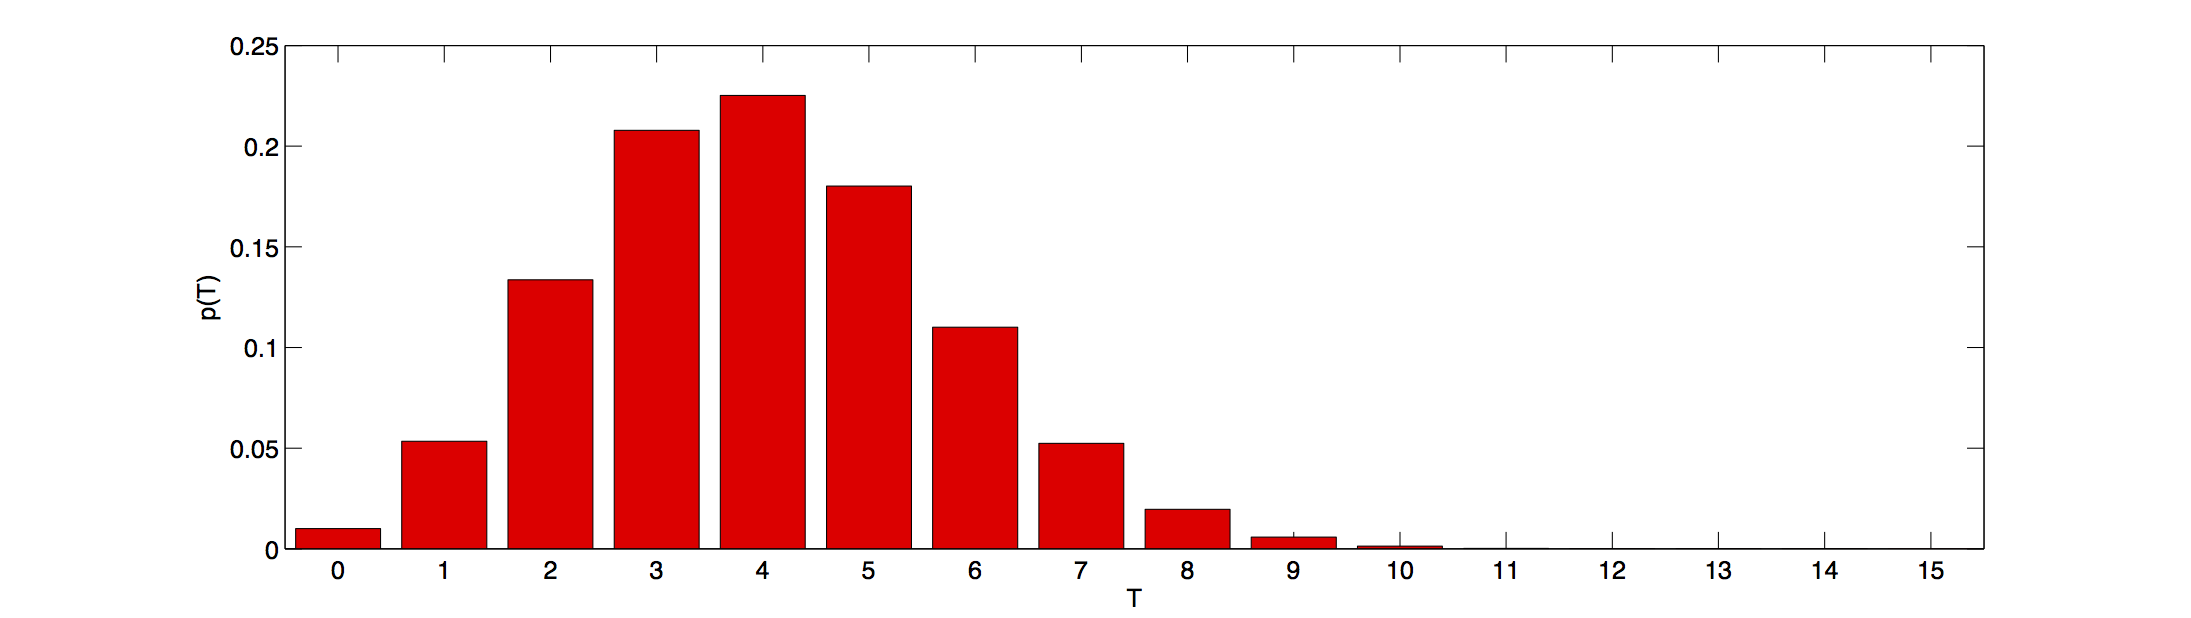
\includegraphics[width=0.65\textwidth]{bin_nonsym.png}
	\end{center}
	
	\vspace{-5pt}
	% -1 здесь из-за дискретности. Если аккуратно все посчитать - выходит действительно, что нужно вычесть единицу
	достигаемый уровень значимости:
	$$p\left(T\right) = \begin{cases}
	1-F_{Bin(n,p_0)}(T-1), & H_1 \colon p>p_0, \\
	F_{Bin(n,p_0)}(T),   & H_1 \colon p<p_0, \\
	\text{через бета-распределение},       & H_1 \colon p\neq p_0. \\
	\end{cases}
	$$
	
\end{frame}


\begin{frame}[label=signtest1]{\hyperlink{classification}{\beamerbutton{(1)}} Одновыборочный критерий знаков}
%%%%%%%%%%%%%%%%%%%%%%%%%%%%%%%%%%%%%%%%%%%%%%%%%%%%%%%%%%%%%%%%%%%%%%%
% Критерии знаков — это одно из семеи?ств непараметрических критериев. Эти критерии обладают невысокои? мощностью, но они краи?не универсальны и практически ничего не требуют от данных, поэтому они очень полезны на практике.
%%%%%%%%%%%%%%%%%%%%%%%%%%%%%%%%%%%%%%%%%%%%%%%%%%%%%%%%%%%%%%%%%%%%%%%
 \only<1>{
 \begin{center}
     \begin{tabular}{rl}
         выборка:                        & $X^n=\left(X_1,\ldots,X_n\right), X_i \neq m_0$         \\
         нулевая гипотеза:               & $H_0\colon \med X = m_0$ \\
         альтернатива:                   & $H_1\colon \med X <\neq> m_0$ \\
         статистика:                     & $T\left(X^n\right) = \sum\limits_{i=1}^n \left[X_i>m_0\right]$\\
         нулевое распределение:          & $Bin(n,\frac1{2})$\\
     \end{tabular}
     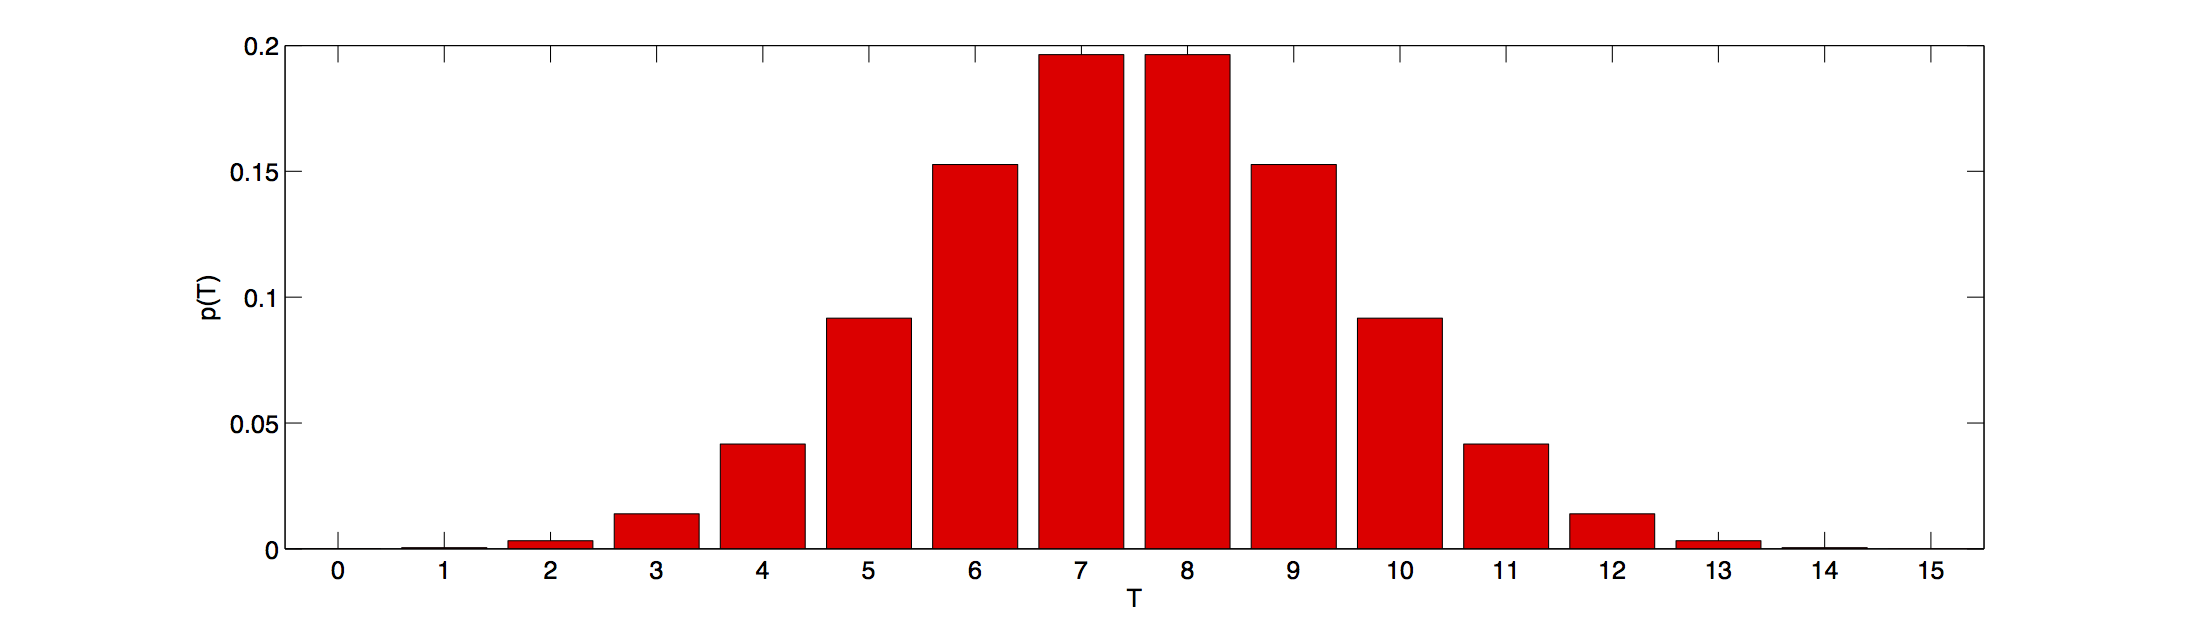
\includegraphics[width=0.8\textwidth]{bin.png}
 \end{center}
  }

  \only<2>{
%%%%%%%%%%%%%%%%%%%%%%%%%%%%%%%%%%%%%%%%%%%%%%%%%%%%%%%%%%%%%%%%%%%%%%%
%Критерии? знаков настолько нетребователен к данным, что его можно использовать даже на цензурированных выборках.
% Пример. Наблюдаются пациенты с лимфоцитарнои? лимфомои?, измеряемыи? признак — это время их жизни в неделях после того, как был поставлен диагноз. Исследование длится семь лет. В выборке есть один пациент, которыи? после семи лет (362 недель наблюдении?) остался жив. Поскольку исследование закончи- лось, неизвестно, сколько еще он прожил после этого. Такая выборка называется цензурированнои? сверху, поскольку на части объектов известна только нижняя граница значения признака.
% Если требуется проверить гипотезу о том, что среднее время дожития составляет 200 недель, против одностороннеи? альтернативы, что оно больше 200 недель, для этои? выборки можно без проблем использовать критерии? знаков. Его достигаемыи? уровень значимости p = 0.9453. То есть нулевую гипотезу нельзя отклонить против одностороннеи? альтернативы.
%%%%%%%%%%%%%%%%%%%%%%%%%%%%%%%%%%%%%%%%%%%%%%%%%%%%%%%%%%%%%%%%%%%%%%%
\begin{block}{Пример,  Dinse, 1982} 
Выживаемость пациентов с лимфоцитарной лимфомой (в~неделях):
 $$49, 58, 75, 110, 112, 132, 151, 276, 281, 362^*$$
 Исследование длилось 7 лет, поэтому для пациентов, проживших дольше, выживаемость неизвестна (выборка цензурирована сверху).
    	
 Превышает ли среднее время дожития 200 недель?
 \end{block}
 \bigskip

 $H_0\colon$ медиана времени дожития не больше 200 недель.

 $H_1\colon$ медиана времени дожития больше 200 недель.
 
 Критерий знаков: $p = 0.9453$.
  }

   	\only<3>{
   \begin{block}{Пример, Shervin, 2004}
     16 лабораторных мышей были помещены в~двухкомнатные клетки, в одной из комнат висело зеркало.
   	Измерялась доля времени, которое каждая мышь проводила в каждой из своих двух клеток.
   	\end{block}
   	\begin{center}
   		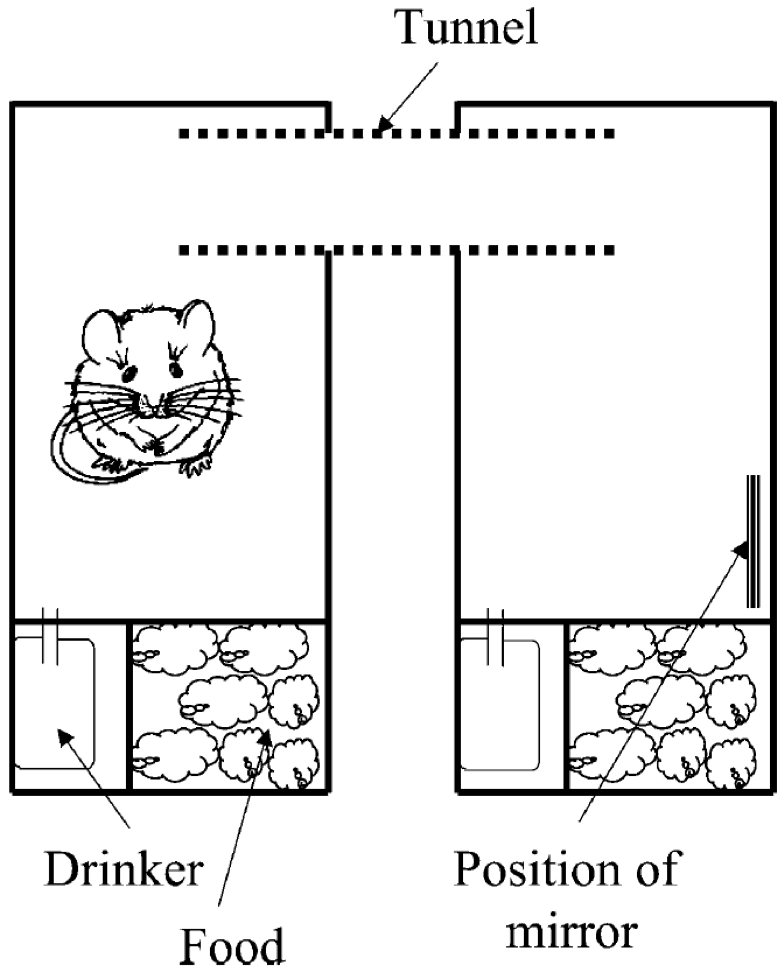
\includegraphics[width=0.2\textwidth]{cage.png}
   	\end{center}
   	
   	Общая постановка:
   	
   	$H_0\colon$ мышам всё равно, висит в клетке зеркало или нет.
   	
   	$H_1\colon$ у мышей есть какие-то предпочтения насчёт зеркала.
   	}
    	
   \only<4>{
	\begin{center}
		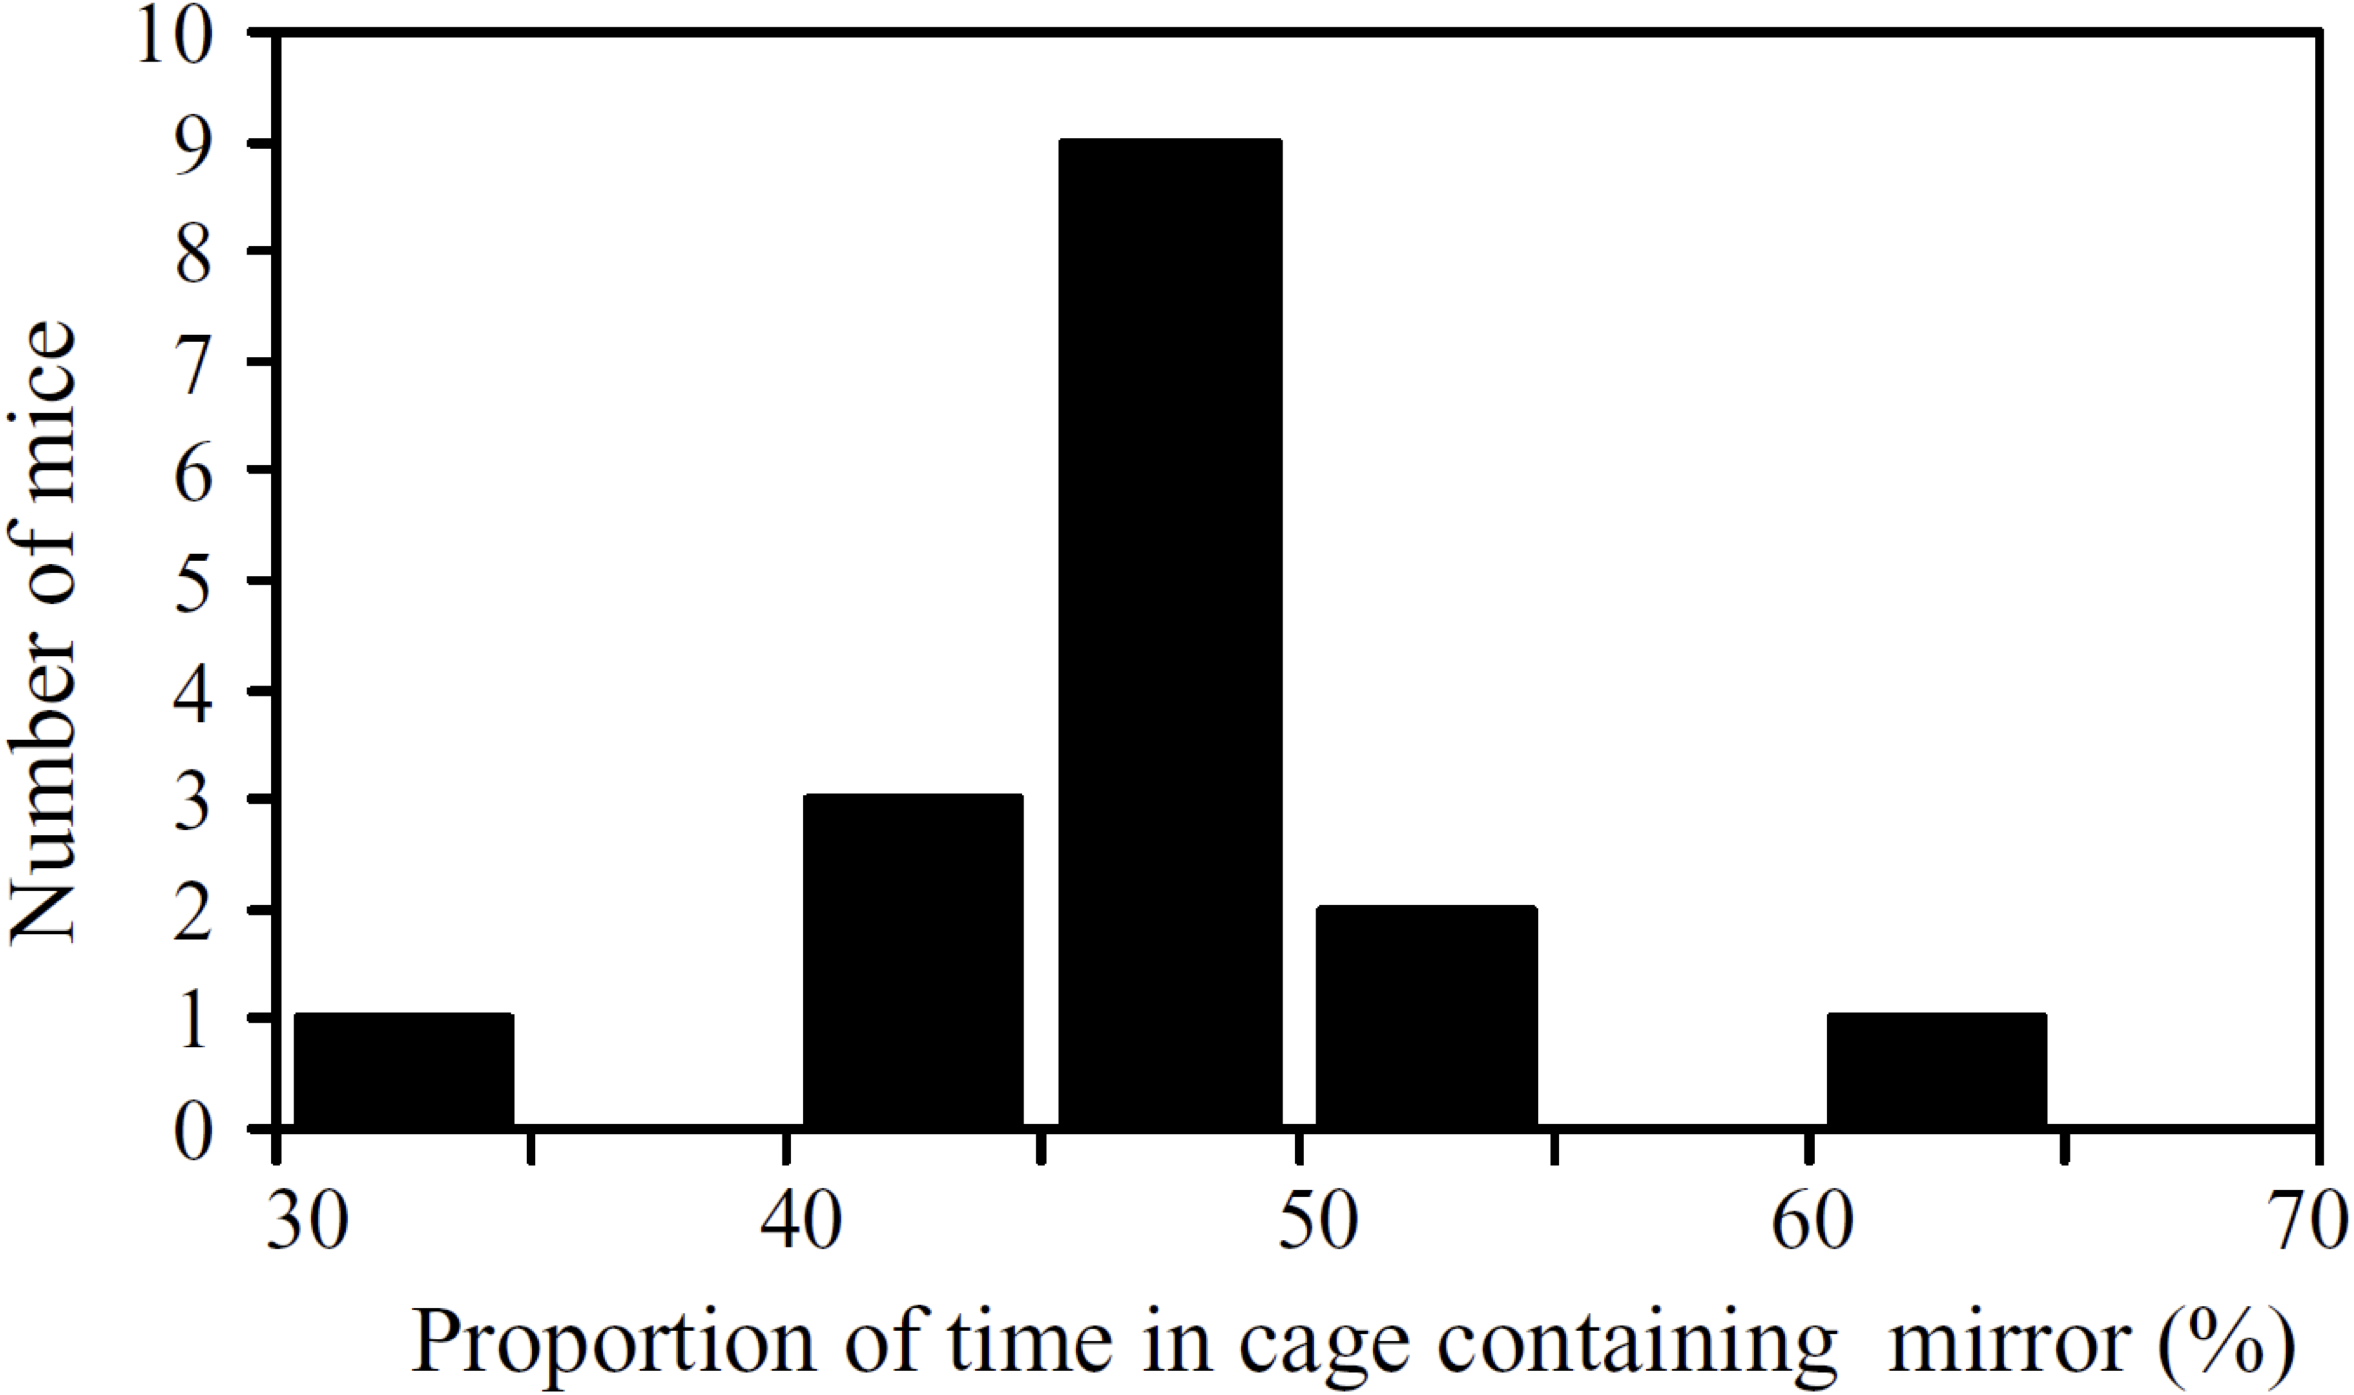
\includegraphics[width=0.7\textwidth]{mouse_hist.png}
	\end{center}
	
	\bigskip
	
	Средняя доля времени, проводимого в клетке с зеркалом~--- $47.6\pm4.7\%.$
	}     	


   \only<5>{
   $H_0\colon$ медиана доли времени, проводимого в клетке с зеркалом, равна~$\frac{1}{2}.$
    	
   $H_1\colon$ медиана доли времени, проводимого в клетке с зеркалом, не~равна~$\frac{1}{2}.$
    	
   \bigskip
    	
   Редуцированные данные: 0~--- мышь провела больше времени в комнате с~зеркалом, 1~--- в комнате без зеркала.
    	
   Статистика: $T$~--- число единиц в выборке.
    	
   \bigskip
    	
   13~из 16~мышей провели больше времени в~комнате без~зеркала.
    	
   \bigskip
    	
   Критерий знаков: $p=0.0213$; доверительный интервал для медианы доли времени, проведённого в комнате с зеркалом:
 \begin{itemize}
	 \item $\left[0.4507, 0.4887\right]$~--- с уровнем доверия 92.32\% 
	 \item $\left[0.4263, 0.4894\right]$~--- с уровнем доверия 97.87\% 
     \item  $\left[0.4389, 0.4890\right]$~--- приближённый 95\% (линейная интерполяция)
 \end{itemize} 
   }
\end{frame}

\subsection{Две выборки}
%%%%%%%%%%%%%%%%%%%%%%%%%%%%%%%%%%%%%%%%%%%%%%%%%%%%%%%%%%%%%%%%%%%%%%%
% В этом уроке иде?т речь о непараметрических критериях, которые проверяют гипотезы о средних, но под «средними» они часто понимают совершенно разные вещи. Так, одновыборочныи? критерии? знаков под средним понимает медиану. Двухвыборочныи? критерии? знаков гипотезу о средних формулирует в представленном выше экзотическом виде. Другие критерии могут использовать другие варианты нулевых гипотез, но, тем не менее, все? это — в каком-то виде утверждение о средних.
% Пример с тополями – тополи использовались для очистки почвы от загрязнения на месте бывшей свалки. Наименьшая концентрация тяжелых металлов была обнаружена в дереве / коре, наибольшая – в листьях старых деревьев -> уборка листьев обязательна :) Сделан вывод, что концентрация тяжелых металлов не влияет на количество древесины. 
%%%%%%%%%%%%%%%%%%%%%%%%%%%%%%%%%%%%%%%%%%%%%%%%%%%%%%%%%%%%%%%%%%%%%%%
\begin{frame}[label=signtest2]{\hyperlink{classification}{\beamerbutton{(2)}} Двухвыборочный критерий знаков}
 \only<1>{
 \begin{center}
    \begin{tabular}{rl}
         выборки:                        & $X_1^n=\left(X_{11},\ldots,X_{1n}\right)$\\
                                         & $X_2^n=\left(X_{21},\ldots,X_{2n}\right), X_{1i} \neq X_{2i}$ \\
                                         & выборки связанные\\
         нулевая гипотеза:               & $H_0\colon \prob\left( X_{1} > X_{2}\right) = \frac1{2}$ \\
         альтернатива:                   & $H_1\colon \prob\left( X_{1} > X_{2}\right) <\neq> \frac1{2}$ \\
         статистика:                     & $T\left(X_1^n, X_2^n\right) = \sum\limits_{i=1}^n \left[X_{1i}>X_{2i}\right]$ \\
         нулевое распределение:          & $Bin(n,\frac1{2})$\\
    \end{tabular}
    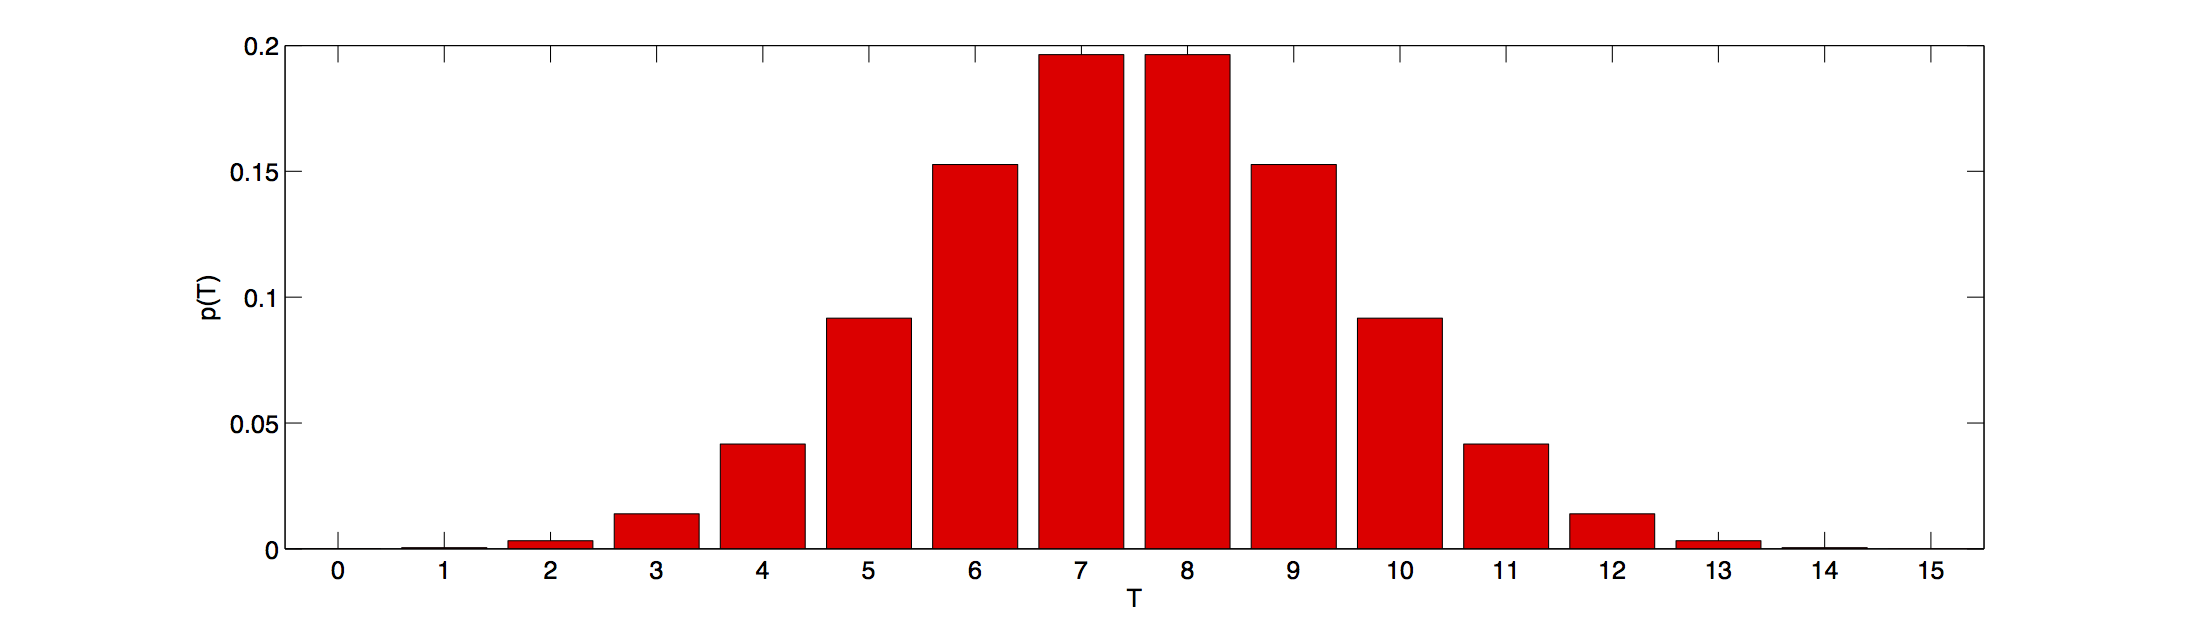
\includegraphics[width=0.8\textwidth]{bin.png}
 \end{center}
 }
  
 \only<2>{
\begin{block}{Пример, Hollander \& Wolfie, 29f}
 Депрессивность 9~пациентов была измерена по шкале Гамильтона до и после первого приёма транквилизатора. Подействовал ли транквилизатор?
 \end{block}
\begin{columns}
\begin{column}{0.4\textwidth}
 \begin{figure}
		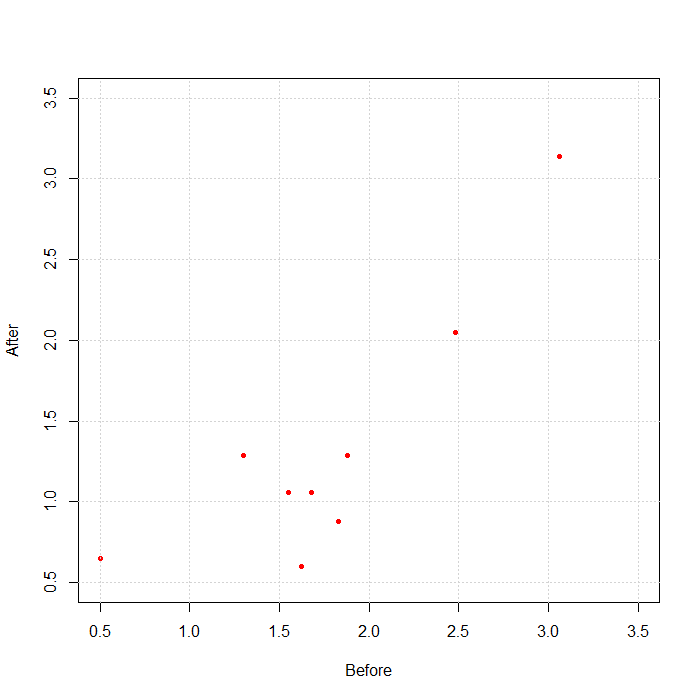
\includegraphics[width=0.8\textwidth]{hamilton.png}
 \end{figure} 
    \end{column}
\begin{column}{0.35\textwidth}
$H_0\colon$ уровень депрессивности не изменился.

 $H_1\colon$ уровень депрессивности снизился.
 	
 	\bigskip
 	
 Критерий знаков: $p = 0.09$, 95\% нижний доверительный предел для медианы изменения~--- $-0.041$.
\end{column}
\end{columns}
	}

	\only<3>{
	\begin{block}{Пример, Laureysens et al., 2004} Для 13 разновидностей тополей, растущих в зоне интенсивного загрязнения, в августе и ноябре измерялась средняя концентрация алюминия в микрограммах на грамм древесины.
	\end{block}
\begin{columns}
\begin{column}{0.35\textwidth}
 \begin{figure}
		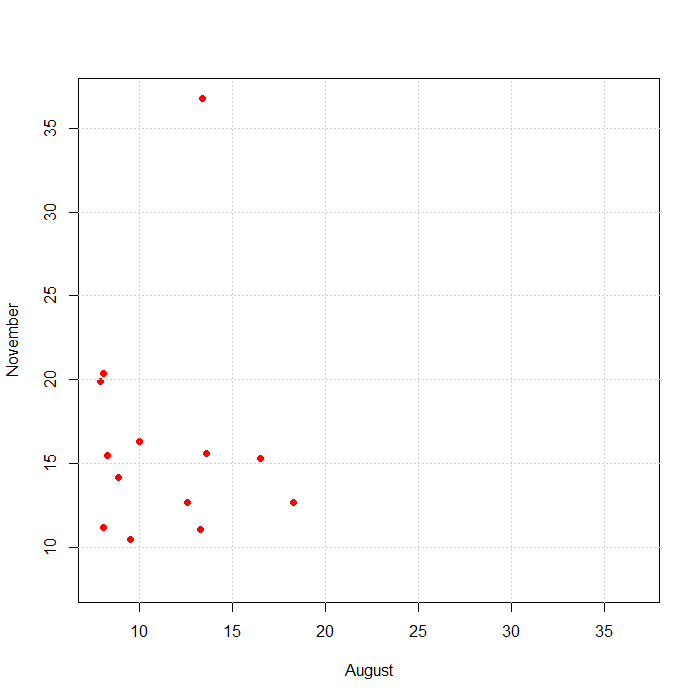
\includegraphics[width=0.8\textwidth]{poplar.png}
 \end{figure} 
   \end{column}
\begin{column}{0.35\textwidth}
	$H_0\colon$ концентрация алюминия не менялась.
		
		$H_1\colon$ концентрация алюминия изменилась.
	
	\bigskip
	
	Для тополей 10 из 13 разновидностей концентрация алюминия увеличилась.
	
	\bigskip
	
	Критерий знаков: $p=0.0923$, 95\% доверительный интервал для медианы изменения~--- $\left[-0.687, 10.107\right].$ 
   \end{column}
   \end{columns}
	}
	
\end{frame}



%%%%%%%%%%%%%%%%%%%%%%%%%%%%%%%%%%%%%%%%%%%%%	%%%%%%%%%%%%%%%%%%%%%%%%%%
% первый пример про комаров --- это когда ты тестируешь эффективность двух репеллентов, намазываешь одних и тех же людей каждым по очереди, выставляешь их в тундру, а потом спрашиваешь, когда они больше страдали
% третий пример про медь – подавляет ли кусок меди в пруду развитие личинок комаров: количество личинок комаров - очень шумная переменная с большой дисперсией, используя критерий знаков, можно искусственно снизить влияние дисперсии на вывод
%%%%%%%%%%%%%%%%%%%%%%%%%%%%%%%%%%%%%%%%%%%%%%%%%%%%%%%%%%%%%%%%%%%%%%%

\begin{frame}{Причины использовать критерий знаков}
 \begin{itemize}
     \item Точные разности $\Delta x_i$ неизвестны, известны только их знаки (сравнение агрессивности комаров).    	
     \bigskip
     \item Разности $\Delta x_i$ при $H_1$ могут быть небольшими по модулю, но иметь систематический характер по знаку (пример с мышами).
     \bigskip
     \item Разности $\Delta x_i$ при $H_0$ могут быть большими по модулю, но случайными но знаку (влияние меди на число личинок комаров).
     \bigskip
 \end{itemize}
\end{frame}



\section{Ранги}
%%%%%%%%%%%%%%%%%%%%%%%%%%%%%%%%%%%%%%%%%%%%%%%%%%%%%%%%%%%%%%%%%%%%%%%
% Для проверки гипотез о средних критерии знаков выбрасывают большую часть информации, содержащуюся в выборке. Вместо исходных значении? признака используется бинарныи? вектор. Ранговые критерии позволяют сохранить больше информации.
% Обратить внимание студентов на дополнительное предположение о симметричности в отличие от критерия знаков --> отсюда возможность отвергнуть нулевую гиптезу из-за несимметричности распределения, а не из-за отличий медианы => дополнительно необходимо проверять семметричность
% Дополнительный плюс методов – можно использовать не только для числовых, но и для ordinal scales, поскольку тествая статистика зависит только от знака и ранга (более экзотично, но тем не менее полезно)
%%%%%%%%%%%%%%%%%%%%%%%%%%%%%%%%%%%%%%%%%%%%%%%%%%%%%%%%%%%%%%%%%%%%%%%
\begin{frame}{Вариационный ряд, ранги, связки}
 $$X_1,\ldots,X_n \;\;\; \Rightarrow \;\;\; X_{(1)}\leq\ldots < \underbrace{X_{(k_1)} = \ldots = X_{(k_2)}}_{\text{связка размера } k_2-k_1+1}<\ldots\leq X_{(n)}$$

 \bigskip

 \textbf{Ранг} наблюдения $X_i$:
%    $$\rank\left(X_i\right)=\mathbb{E}\left\{r\left|X_i=X_{(r)}\right.\right\}$$
%    т.\,е.  

 если $X_i$ не в связке, то $\rank\left(X_i\right)=r\colon X_i=X_{(r)}$, \\
%    \hspace{14pt} 
 если $X_i$ в связке $X_{(k_1)}, \ldots, X_{(k_2)}$, то $\rank\left(X_i\right)=\frac{k_1+k_2}{2}.$
\end{frame}

\subsection{Одна выборка}
\begin{frame}[label=signrank1]{\hyperlink{classification}{\beamerbutton{(3)}} Одновыборочный критерий знаковых рангов Уилкоксона}
 \only<1>{
   \begin{center}
     \begin{tabular}{rl}
         выборка:                        & $X^n=\left(X_1,\ldots,X_n\right), X_i \neq m_0$\\
					            & $F\left(X\right)$ симметрично относительно медианы\\
         нулевая гипотеза:               & $H_0\colon \med X = m_0$ \\
         альтернатива:                   & $H_1\colon \med X <\neq> m_0$ \\
         статистика:                     & $W\left(X^n\right) = \sum\limits_{i=1}^n \rank\left(\left|X_i - m_0\right|\right)\cdot \sign\left(X_i - m_0\right)$ \\
         нулевое распределение:          & табличное\\
     \end{tabular}
     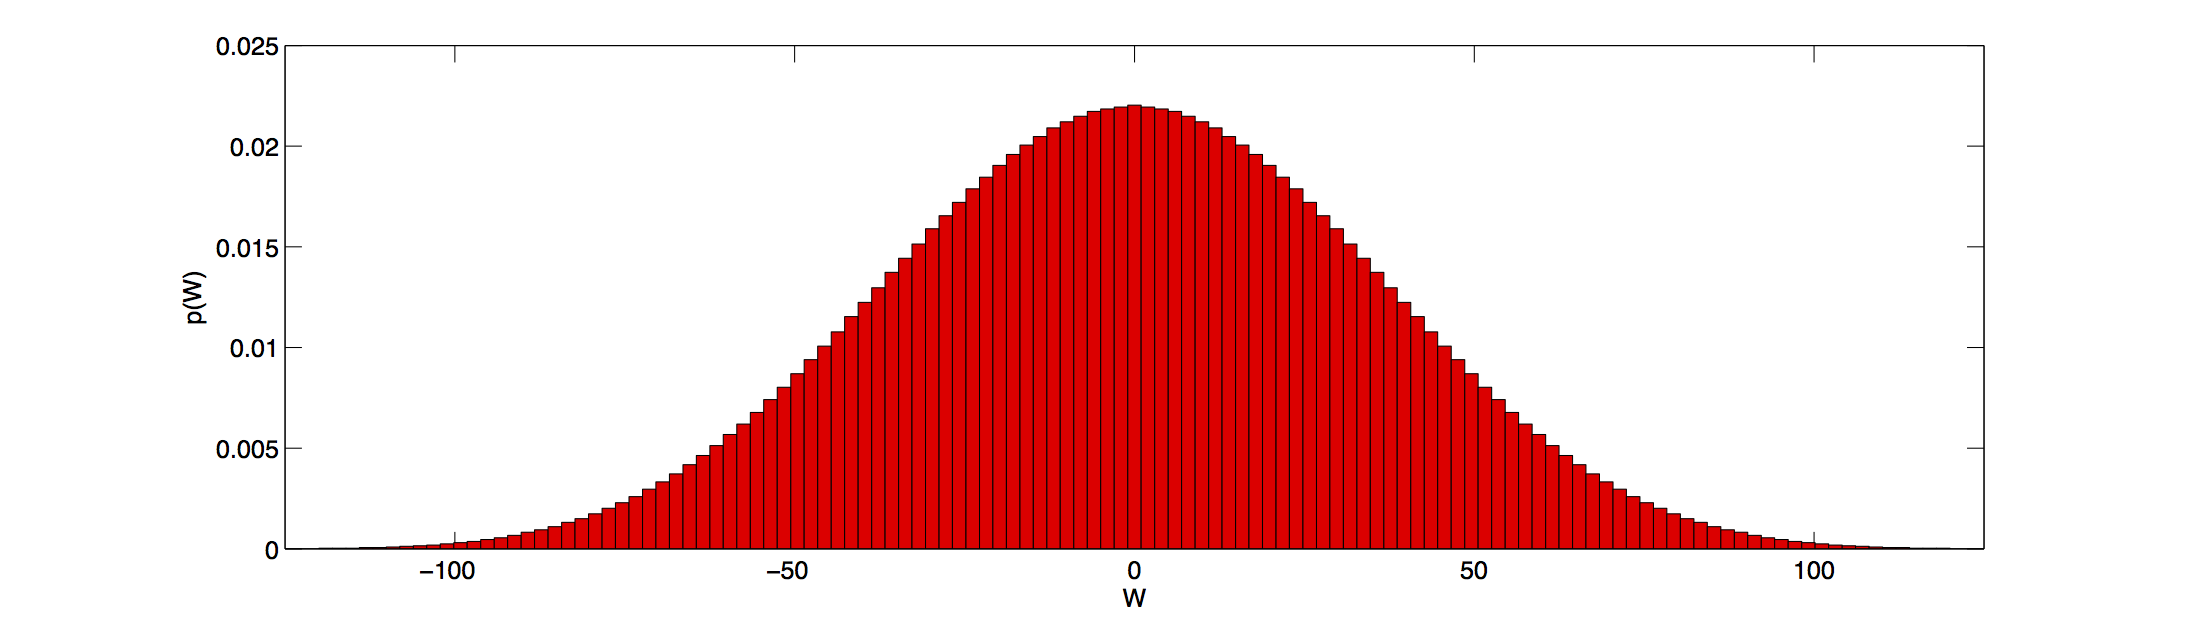
\includegraphics[width=0.8\textwidth]{signrank.png}
 \end{center}
 }

 \only<2>{
%%%%%%%%%%%%%%%%%%%%%%%%%%%%%%%%%%%%%%%%%%%%%%%%%%%%%%%%%%%%%%%%%%%%%%%
% При справедливости нулевои? гипотезы каждыи? из рангов в выборке мог с одинаковои? вероятностью реализоваться с любым знаком (sign(Xi ? m0)): и с «+», и с «?». Таким образом, получается 2n вариантов распределения знаков по рангам. Перебирая все эти варианты, для каждого из них можно вычислить значение статистики, пример перебора показан в таблице. Именно так строится нулевое распределение критерия знаковых рангов.
%%%%%%%%%%%%%%%%%%%%%%%%%%%%%%%%%%%%%%%%%%%%%%%%%%%%%%%%%%%%%%%%%%%%%%%
 Откуда берётся табличное распределение?

 \bigskip

    \begin{center}  \setlength{\tabcolsep}{5pt}
        \begin{tabular}{c c c c c c c c c c c}
        $1$&$2$&$3$&$4$&$5$&$W$\\
        $-$&$-$&$-$&$-$&$-$&$-15$\\
        $+$&$-$&$-$&$-$&$-$&$-13$\\
        $-$&$+$&$-$&$-$&$-$&$-11$\\
        $+$&$+$&$-$&$-$&$-$&$-9$\\
        $-$&$-$&$+$&$-$&$-$&$-9$\\
        \dots&\dots&\dots&\dots&\dots&\dots\\
         $+$&$+$&$-$&$+$&$+$&$9$\\
        $-$&$-$&$+$&$+$&$+$&$9$\\
        $+$&$-$&$+$&$+$&$+$&$11$\\
        $-$&$+$&$+$&$+$&$+$&$13$\\
        $+$&$+$&$+$&$+$&$+$&$15$\\
        \end{tabular}
    \end{center}
    
    Всего $2^n$ вариантов.
 }
    \only<3>{
    $n=5$:
    
    \begin{center}
        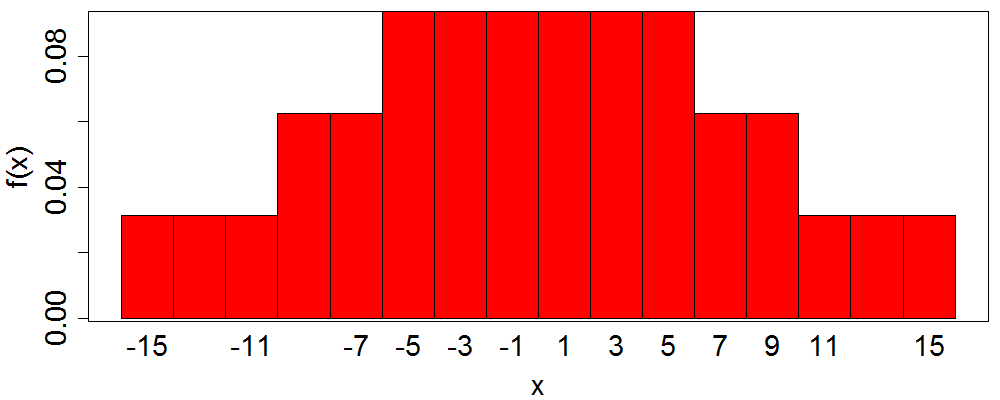
\includegraphics[width=0.8\textwidth]{ranksum5.png}    
    \end{center}
    }
    \only<4>{
    $n=10$:
    
    \begin{center}
        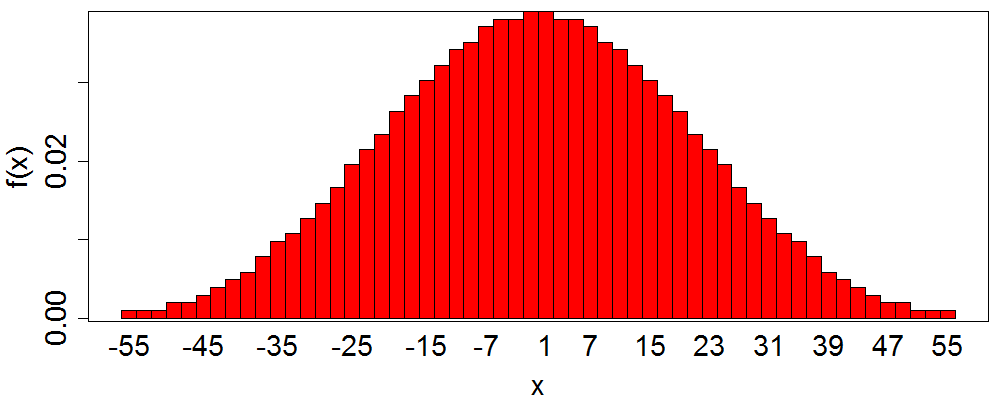
\includegraphics[width=0.8\textwidth]{ranksum10.png}    
    \end{center}
    }   
\only<5>{    
    $n=15$:
    
    \begin{center}
        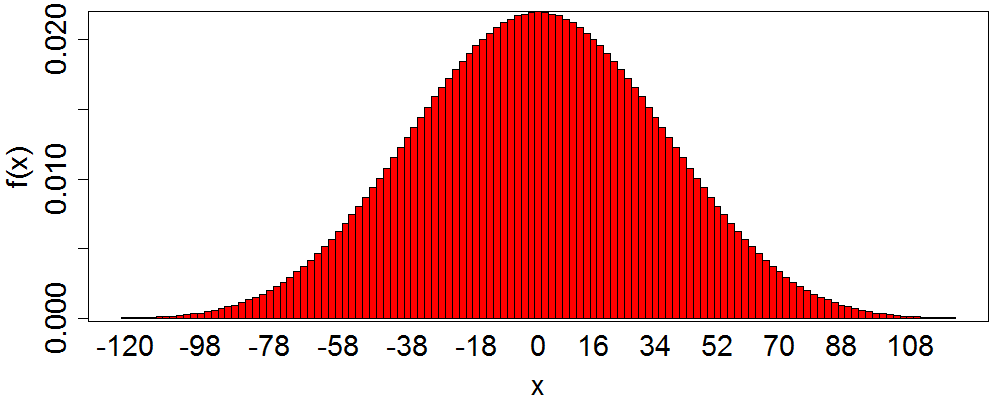
\includegraphics[width=0.8\textwidth]{ranksum15.png}    
    \end{center}   

    \bigskip
       
    Аппроксимация для $n>20$:
    $$W\approx \sim N\left(0, \frac{n(n+1)(2n+1)}{6}\right).$$     
    }
 \only<6>{
 \textbf{Пример 1} (Bonnini, табл. 1.4): диаметры шайб на производстве ($n=24$):
 
     \begin{center}        
         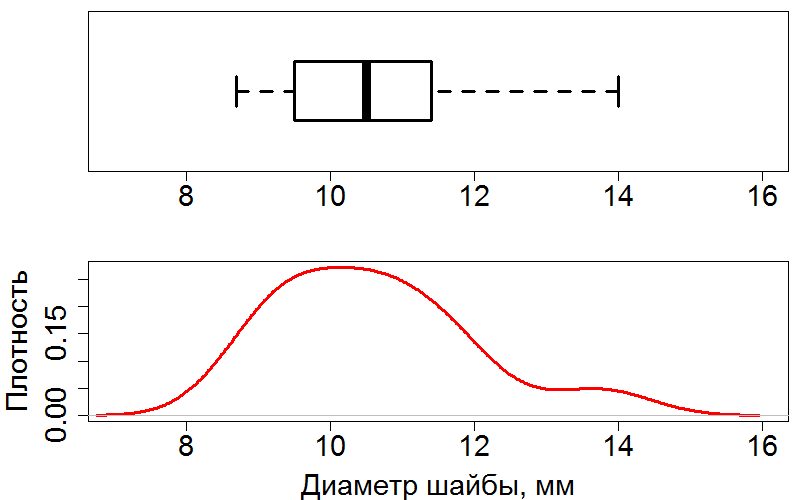
\includegraphics[width=0.4\textwidth]{washer.png}
     \end{center}
     
     Соответствуют ли шайбы стандартному размеру 10 мм?
 
 \bigskip

	$H_0\colon$ средний диаметр шайбы~--- $10$ мм, $\med X = 10$.
	
	$H_1\colon$ средний диаметр шайбы не соответствует стандарту, $\med X\neq10$.
	
	\bigskip
	
	Критерий знаковых рангов: $p=0.0673$, выборочная медиана диаметра~--- $10.5$~мм ($95$\% доверительный интервал~---  $\left[9.95, 11.15\right]$~мм).
 }
 
 \only<7>{
 \textbf{Пример 2} (зеркала в клетках мышей):\\
 \bigskip
 $H_0\colon$ медиана доли времени, проводимого в клетке с зеркалом, равна~$\frac{1}{2}.$

 $H_1\colon$ медиана доли времени, проводимого в клетке с зеркалом, не~равна~$\frac{1}{2}$.\\
  \bigskip
  Критерий знаковых рангов: $p=0.0934.$    
 }
\end{frame}

\subsection{Две выборки}
\begin{frame}[label=signrank2]{\hyperlink{classification}{\beamerbutton{(4)}} Критерий знаковых рангов Уилкоксона для связанных выборок}
%%%%%%%%%%%%%%%%%%%%%%%%%%%%%%%%%%%%%%%%%%%%%%%%%%%%%%%%%%%%%%%%%%%%%%%
% Как и до этого в курсе, двухвыборочная задача со связанными выборками решается с использованием того же самого критерия, что и одновыборочная.
%%%%%%%%%%%%%%%%%%%%%%%%%%%%%%%%%%%%%%%%%%%%%%%%%%%%%%%%%%%%%%%%%%%%%%%
 \only<1>{
   \begin{center}
     \begin{tabular}{rl}
         выборки:                        & $X_1^n=\left(X_{11},\ldots,X_{1n}\right)$         \\
                                         & $X_2^n=\left(X_{21},\ldots,X_{2n}\right), X_{1i} \neq X_{2i}$ \\
                                         & выборки связанные, разность выборок симметрична относительно медианы\\
         нулевая гипотеза:               & $H_0\colon \med \left(X_{1} - X_{2}\right)=0$ \\
         альтернатива:                   & $H_1\colon \med \left(X_{1} - X_{2}\right) <\neq> 0$ \\
         статистика:                     & $W\!\left(X_1^n, X_2^n\right)\! = \!\!\sum\limits_{i=1}^n \!\rank\!\left(\left|X_{1i} - X_{2i}\right|\right)\cdot \sign\!\left(X_{1i} - X_{2i}\right)$ \\
         нулевое распределение:          & табличное\\
     \end{tabular}
     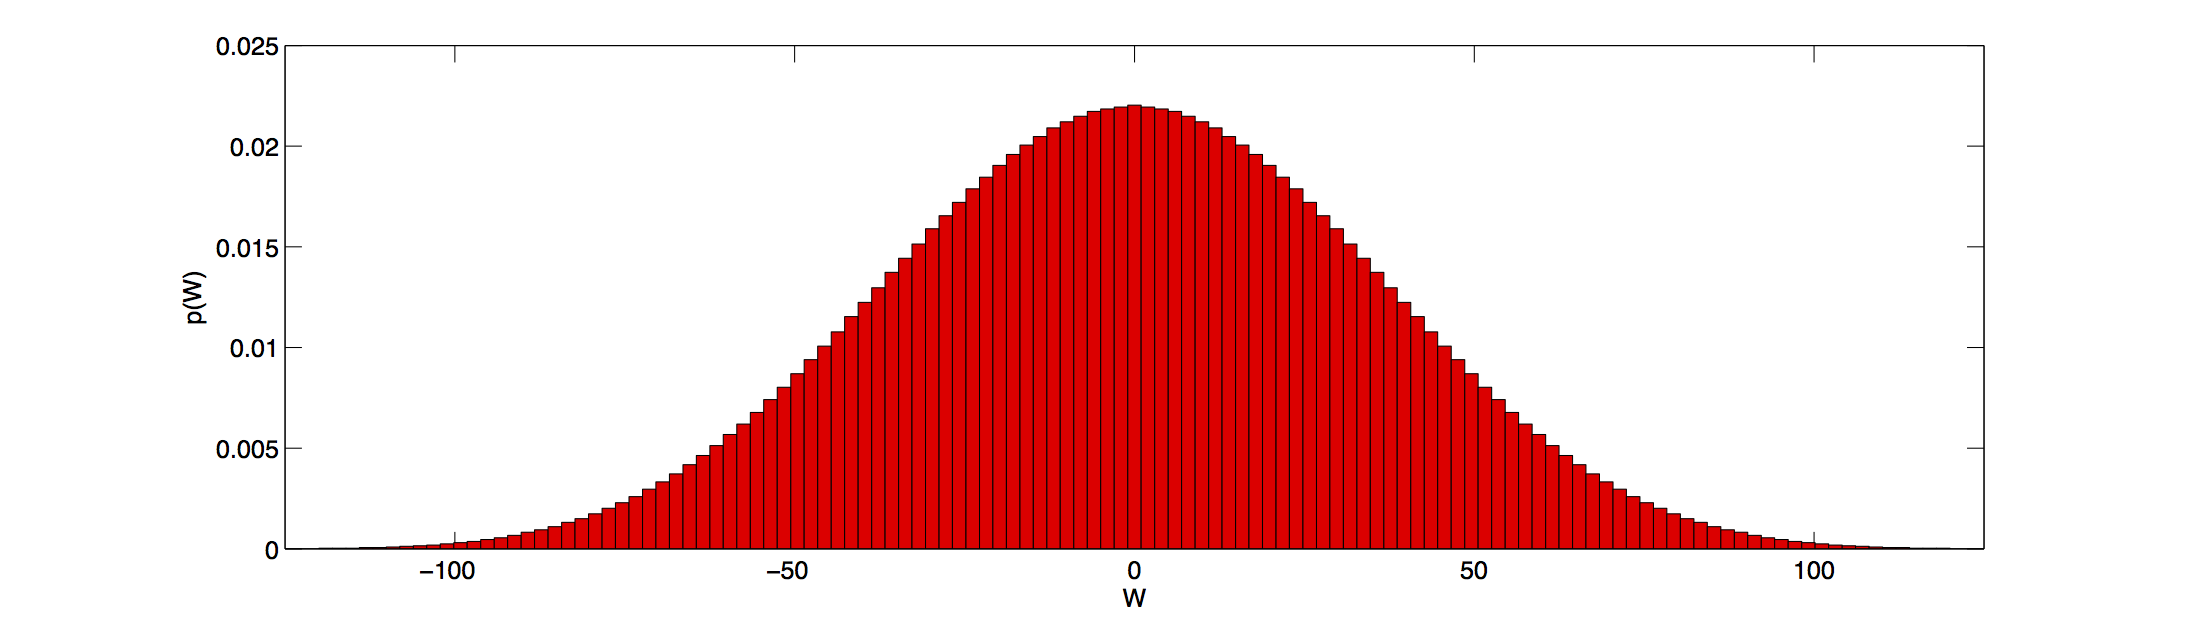
\includegraphics[width=0.8\textwidth]{signrank.png}
 \end{center}
 }

 \only<2>{
 \begin{block}{Пример, Kanji, критерий 48} Управляемый вручную станок на каждом шаге процесса производит пару пружин. Для 14~пар измерена прочность:
 \begin{align*}
 X_1\colon & \{1.38,  0.39, 1.42, 0.54, 5.94, 0.59, 2.67, 2.44, 0.56, 0.69, 0.71, 0.95, 0.50, 9.69\}, \\
 X_2\colon & \{1.42, 0.39, 1.46, 0.55, 6.15, 0.61, 2.69, 2.68, 0.53, 0.72, 0.72, 0.93, 0.53, 10.37\}.
 \end{align*}
 Одинакова ли прочность пружин в паре?
 \end{block}
 \bigskip

 $H_0\colon$ средние значение прочности пружин в паре равны.

 $H_1\colon$ средние значение прочности пружин в паре не равны $ \Rightarrow p = 0.0142$, 95\% доверительный интервал для медианной разности~--- $\left[0.005, 0.14\right].$
 }
 
 \only<3>{
 \textbf{Пример 2} (алюминий в тополях):\\
 \bigskip
 
 $H_0\colon$ медиана изменения концентрации алюминия равна нулю.

 $H_1\colon$ медиана изменения концентрации алюминия не~равна нулю $\Rightarrow 0.0398,$ 95\% доверительный интервал для медианы изменения~--- $\left[0.35, 9.3\right].$ 
 }    
\end{frame}

\begin{frame}[label=mannwhitney]{\hyperlink{classification}{\beamerbutton{(5)}} Критерий Манна-Уитни-Уилкоксона}
 \only<1>{
%%%%%%%%%%%%%%%%%%%%%%%%%%%%%%%%%%%%%%%%%%%%%%%%%%%%%%%%%%%%%%%%%%%%%%%
% Относительно параметра ? альтернатива в этом критерии может быть одностороннеи? или двустороннеи?. Если справедлива альтернативная гипотеза и между распределениями деи?ствительно есть сдвиг, то средние значения признаков в выборках будут различаться. Поэтому это тоже в каком-то виде гипотеза о средних.
%%%%%%%%%%%%%%%%%%%%%%%%%%%%%%%%%%%%%%%%%%%%%%%%%%%%%%%%%%%%%%%%%%%%%%%
   \begin{center}
     \begin{tabular}{rl}
         выборки:                        & $X_1^{n_1}=\left(X_{11},\ldots,X_{1n_1}\right)$         \\
                                         & $X_2^{n_2} = \left(X_{21},\ldots,X_{2n_2}\right)$ \\ 
                                         & выборки независимые\\
         нулевая гипотеза:               & $H_0\colon F_{X_1}\left(x\right) = F_{X_2}\left(x\right)$ \\
         альтернатива:                   & $H_1\colon F_{X_1}\left(x\right) = F_{X_2}\left(x+\Delta\right), \Delta <\neq> 0$ \\
         статистика:                     & $X_{(1)}\leq\ldots\leq X_{(n_1+n_2)}$ --- вариационный ряд \\
                                         & объединённой выборки $X = X_1^{n_1} \bigcup X_2^{n_2}$ \\
                                         & $R_1\left(X_1^{n_1}, X_2^{n_2}\right) = \sum\limits_{i=1}^{n_1} \rank\left(X_{1i}\right)$ \\
         нулевое распределение:          & табличное\\
     \end{tabular}
     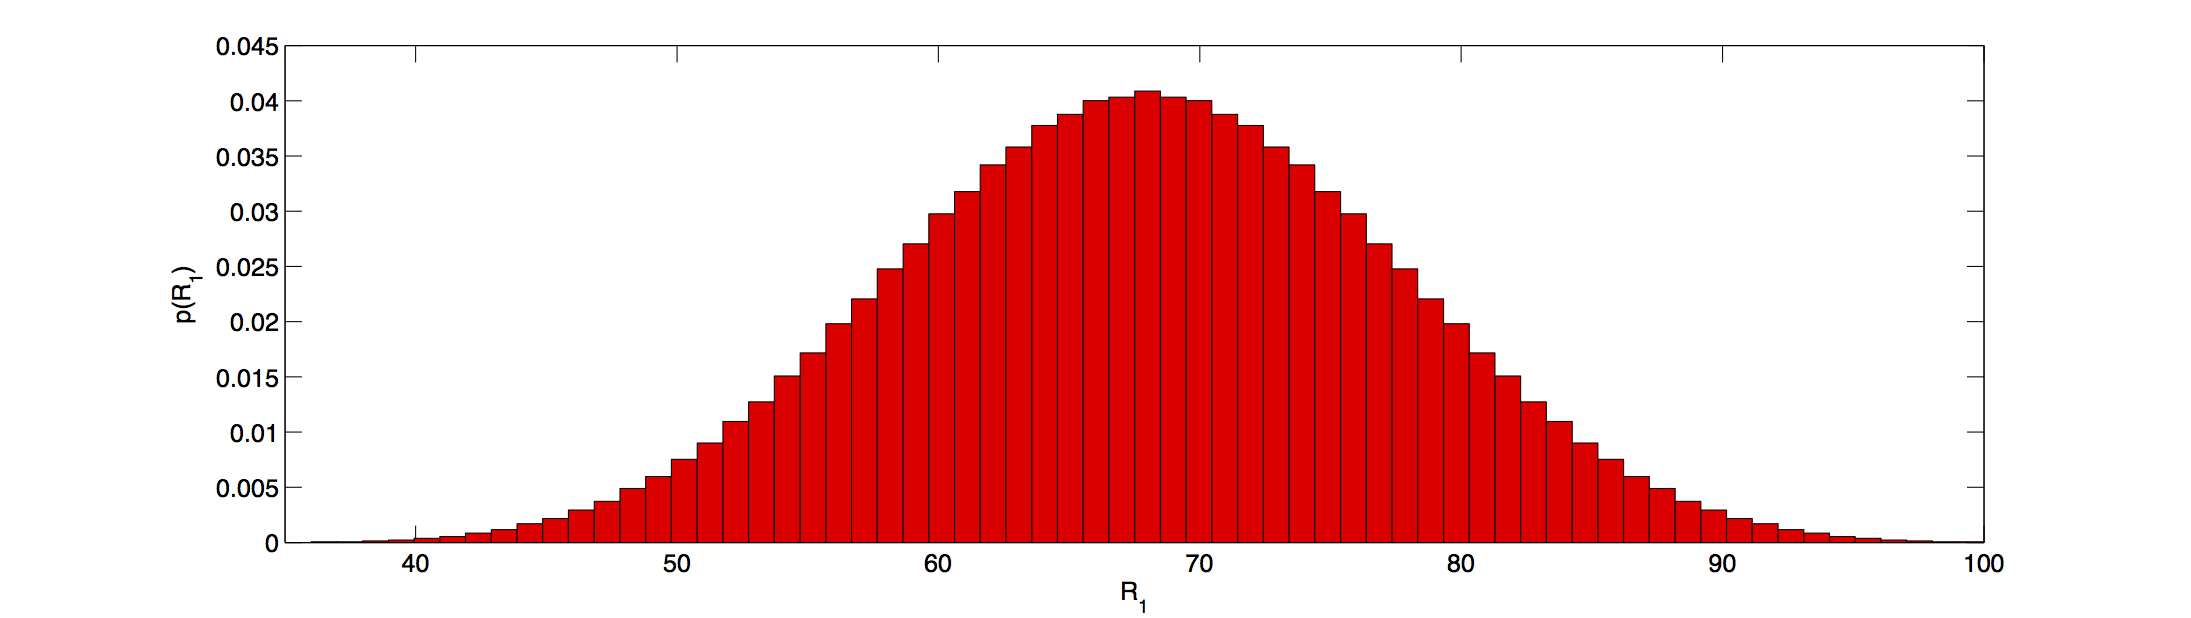
\includegraphics[width=0.8\textwidth]{mann.png}
 \end{center}
 }
 \only<2>{
%%%%%%%%%%%%%%%%%%%%%%%%%%%%%%%%%%%%%%%%%%%%%%%%%%%%%%%%%%%%%%%%%%%%%%%
% Нулевое распределение этои? статистики, как и в предыдущем случае, табличное. Оно получается следующим образом. Если нулевая гипотеза справедлива, то каждыи? из рангов с одинаковои? вероятностью мог реализоваться как в выборке X1, так и в выборке X2. Необходимо перебрать все возможные варианты того, как это могло произои?ти, всего таких вариантов n1. На каждом из этих вариантов нужно вычислить n1+n2 значение статистики критерия Манни-Уитни, так и получается нулевое распределение.
%%%%%%%%%%%%%%%%%%%%%%%%%%%%%%%%%%%%%%%%%%%%%%%%%%%%%%%%%%%%%%%%%%%%%%%
 Откуда берётся табличное распределение?

 \bigskip

    \begin{center}
    	\begin{tabular}{c c c}
    		$X_1$ & $X_2$  & $R_1$\\
    		\{1,2,3\}      & \{4,5,6,7\}     & 6 \\
    		\{1,2,4\}      & \{3,5,6,7\}     & 7 \\
    		\{1,2,5\}      & \{3,4,6,7\}     & 8 \\
    		\{1,2,6\}      & \{3,4,5,7\}     & 9 \\
    		\{1,2,7\}      & \{3,4,5,6\}     & 10 \\
    		\{1,3,4\}      & \{2,5,6,7\}     & 8 \\
    		\dots&\dots&\dots\\
    		\{3,5,7\}      & \{1,2,4,6\}     & 15 \\
    		\{3,6,7\}      & \{1,2,4,5\}     & 16 \\
    		\{4,5,6\}      & \{1,2,3,7\}     & 15 \\
    		\{4,5,7\}      & \{1,2,3,6\}     & 16 \\
    		\{4,6,7\}      & \{1,2,3,5\}     & 17 \\
    		\{5,6,7\}      & \{1,2,3,4\}     & 18 \\
    	\end{tabular}
    \end{center}	
        
    Всего $C_{n_1+n_2}^{n_1}$ вариантов.
 }

   \only<3>{
    	$n_1=n_2=5$:
    	
    	\begin{center}
    		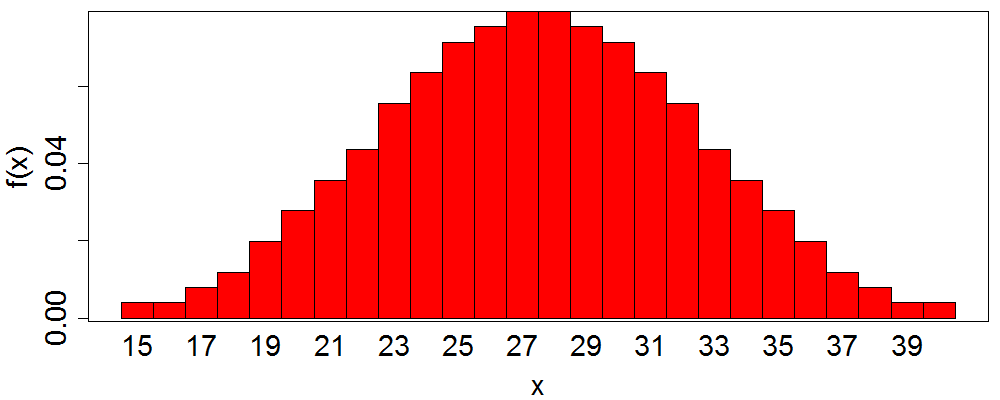
\includegraphics[width=0.8\textwidth]{MU5-5.png}    
    	\end{center}
    }
    \only<4>{
    	$n_1=n_2=10$:
    	
    	\begin{center}    		
    		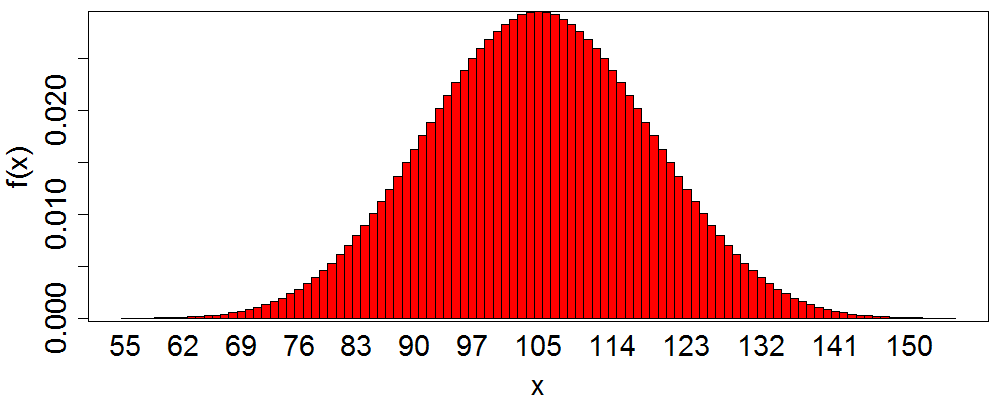
\includegraphics[width=0.8\textwidth]{MU10-10.png}    
    	\end{center}

    	\bigskip
    	
    	Аппроксимация для $n_1,n_2>10$:
    	$$R_1\sim N\left(\frac{n_1(n_1+n_2+1)}{2}, \frac{n_1n_2(n_1+n_2+1)}{12}\right).$$  
    }	

 \only<5>{
    \begin{block} {Пример, Kanji, критерий 52} Cотрудник налоговой службы хочет сравнить средние значения в~двух выборках заявленных трат на компенсацию командировочных расходов в одной и той же компании в~двух разных периодах (расходы скорректированы на инфляцию).
 \begin{align*}
 X_1\colon & \{50.5, 37.5, 49.8, 56.0, 42.0, 56.0, 50.0, 54.0, 48.0\}, \\
 X_2\colon & \{57.0, 52.0, 51.0, 44.2, 55.0, 62.0, 59.0, 45.2, 53.5, 44.4\}.
 \end{align*}
 Равны ли средние расходы?
\end{block}
 \bigskip

 $H_0\colon$ средние расходы равны.

 $H_1\colon$ средние расходы не равны $ \Rightarrow p = 0.3072$, 95\% доверительный интервал для медианной разности~--- $\left[-9, 4\right]$.
 }
 
 
%%%%%%%%%%%%%%%%%%%%%%%%%%%%%%%%%%%%%%%%%%%%%%%%%%%%%%%%%%%%%%%%%%%%%%%
% В этои? задаче измеряемыи? признак — это респираторныи? обмен, соотношение числа молекул углекислого газа и кислорода в выдыхаемом воздухе. Респираторныи? обмен является косвенным признаком того, из чего в данныи? момент мышцы вырабатывают энергию, из жиров или углеводов. В эксперименте измеряется респираторныи? обмен у 18 испытуемых в процессе физических упражнении?. За час до этого 9 из
% 8 них получили таблетку кофеина, а оставшиеся 9 — таблетку плацебо. Хочется понять, повлиял ли кофеин на среднее значение показателей респираторного обмена.
% большое значение коэффициента означает, что окисалюятся углеводы, малый – жиры
%%%%%%%%%%%%%%%%%%%%%%%%%%%%%%%%%%%%%%%%%%%%%%%%%%%%%%%%%%%%%%%%%%%%%%% 
\only<6>{
RER~--- соотношение числа молекул $CO_2$ и $O_2$ в~выдыхаемом воздухе. 

В эксперименте измерялся респираторный обмен $18$ испытуемых в~процессе физических упражнений. За час до этого $9$ из них получили таблетку кофеина, $9$~--- плацебо.
	
	\begin{figure}
		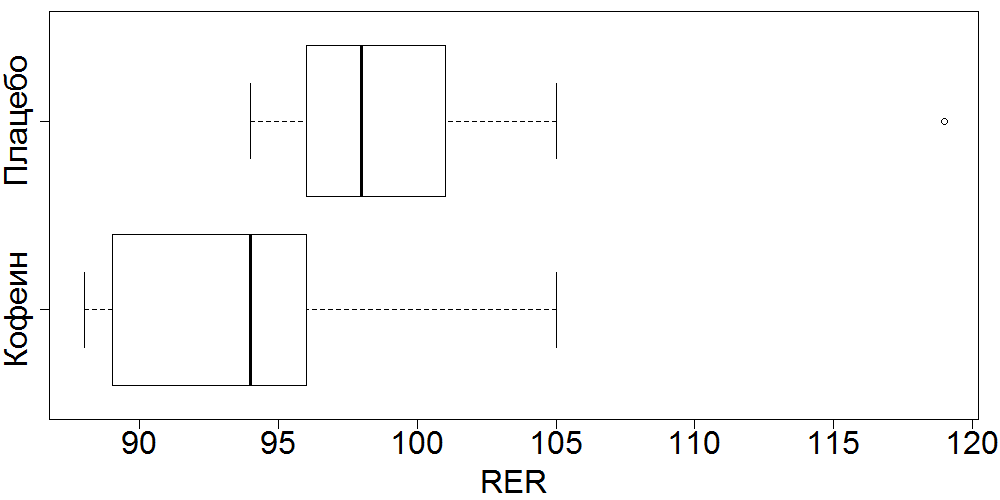
\includegraphics[width=0.4\textwidth]{rer.png}
	\end{figure} 	

Повлиял ли кофеин на значение RER?
 
 \bigskip
 $H_0\colon$ среднее значение показателя респираторного обмена не отличается в~двух группах.

 $H_1\colon$ среднее значение показателя респираторного обмена отличается в~двух группах.
 }
 
 \only<7>{
  \begin{center}
     \begin{tabular}{|c| c| c| c| c|} \hline
     Ранг & Наблюдение & Номер наблюдения & Наблюдение & Ранг\\ \hline
     16.5 & 105 & 1 & 96  & 9   \\
     18   & 119 & 2 & 99  & 13  \\
     14   & 100 & 3 & 94  & 5.5 \\
     11   & 97  & 4 & 89  & 3   \\
     9    & 96  & 5 & 96  & 9   \\
     15   & 101 & 6 & 93  & 4   \\
     5.5  & 94  & 7 & 88  & 1.5 \\
     7    & 95  & 8 & 105 & 16.5\\
     12   & 98  & 9 & 88  & 1.5 \\ \hline
     \end{tabular}
  \end{center}

  \bigskip

  Статистика $R_1$ "--- сумма рангов в одной из групп.

  \bigskip

  $p=0.0521,$ сдвиг между средними~--- $6$~пунктов, ($95$\% доверительный интервал~---  $\left[-0.00005, 12\right]$~пт).
 }
\end{frame}

\begin{frame}[label=siegel]{\hyperlink{classification}{\beamerbutton{(6)}} Критерий Ансари-Брэдли}
    \only<1>{\small
      \begin{center} 
        \begin{tabular}{rl}
            выборки:                        & $X_1^{n_1}=\left(X_{11},\ldots,X_{1n_1}\right)$ \\
                                            & $X_2^{n_2}=\left(X_{21},\ldots,X_{2n_2}\right)$ \\
                                            & выборки независимые, $ \med(X_1) = \med(X_2) $ \\
%                                            &  \\
            нулевая гипотеза:               & $H_0\colon \mathbb{D} X_{1} = \mathbb{D} X_{2}$ \\
            альтернатива:                   & $H_1\colon \mathbb{D} X_{1} <\neq> \mathbb{D} X_{2}$ \\
            статистика:                     & $X_{(1)}\leq\ldots\leq X_{(N)}$ --- вариационный ряд \\
                                            & объединённой выборки $X^N = X_1^{n_1} \bigcup X_2^{n_2}, N=n_1+n_2$ \\
                                            & $R_1\left(X_1^{n_1}, X_2^{n_2}\right) = \sum\limits_{i=1}^{n_1} \widetilde{\rank}\left(X_{1i}\right)$ \\
            нулевое распределение:          & табличное\\
        \end{tabular}
        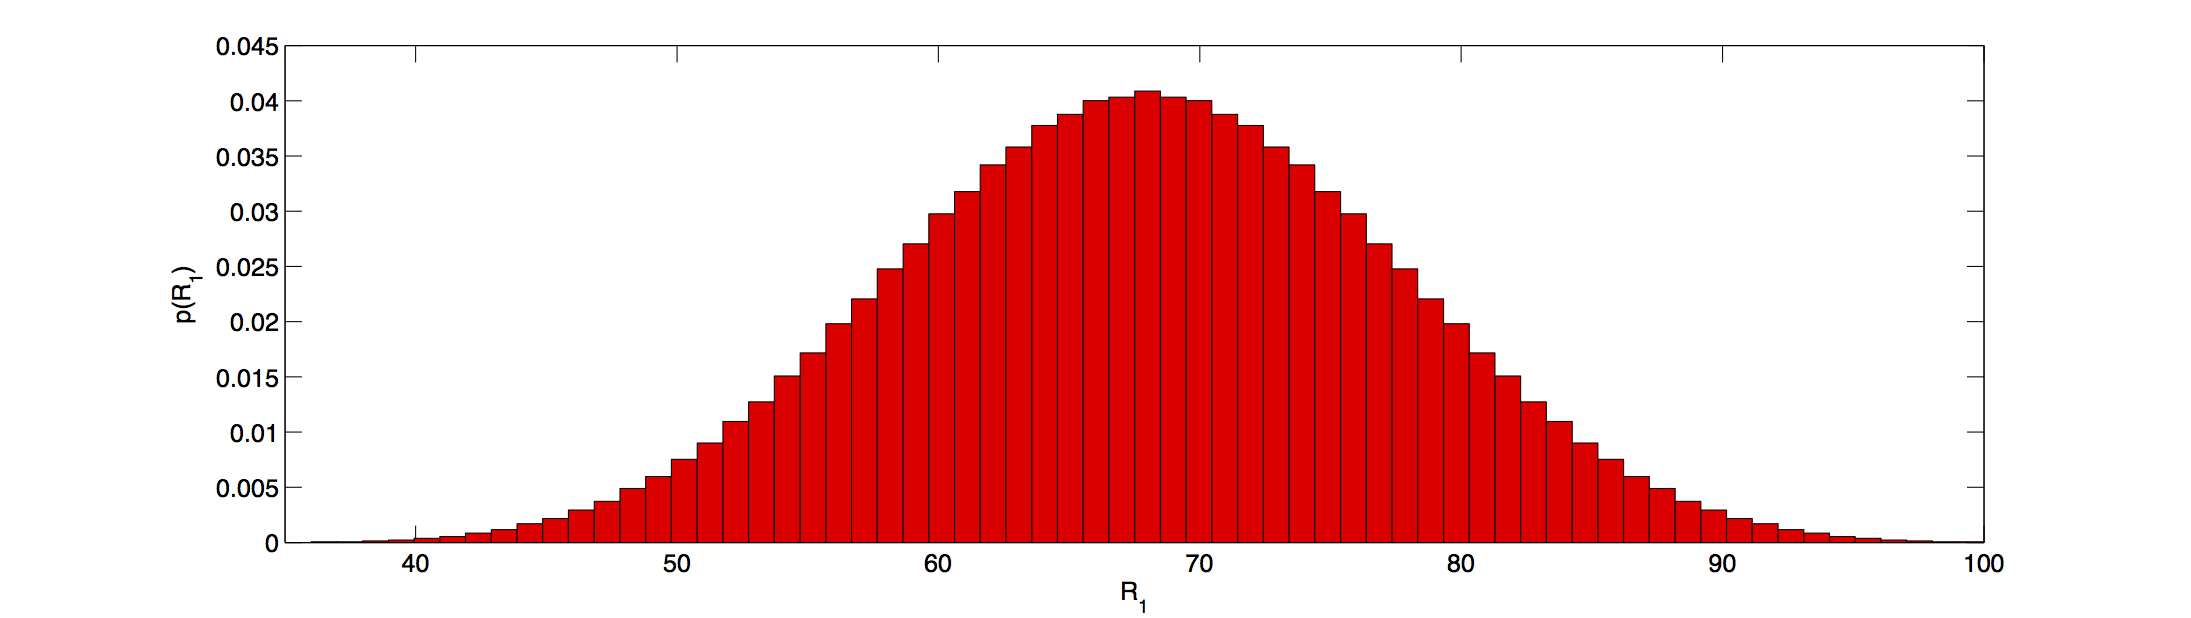
\includegraphics[width=0.8\textwidth]{mann.png}
    \end{center}
     Ранги присваиваются от краёв к центру:
      \begin{center}\setlength{\tabcolsep}{2pt}
        \begin{tabular}{cccccccccccccc}
        $X_{(i)}$                       & $X_{(1)}$ &$\leq$& $X_{(2)}$ &$\leq$& $X_{(3)}$ &$\leq$& $\ldots$ &$\leq$ &$X_{(N-2)}$ &$\leq$& $X_{(N-1)}$ &$\leq$& $X_{(N)}$ \\
        $\widetilde{\rank}\left(X_{(i)}\right)$ & 1         &      &  2        &      & 3         &      &          &       & 3          &      &    2        &      & 1
        \end{tabular}
          \end{center}
    }

    \only<2>{
    \begin{block} {Пример,Bonnini, табл. 2.1} Два поставщика шестнадцатикилограммовых свинцовых слитков выслали по выборке образцов. Средний вес образцов в~обеих выборках соответствует норме; различаются ли дисперсии?
    \end{block}
    \begin{figure}
    	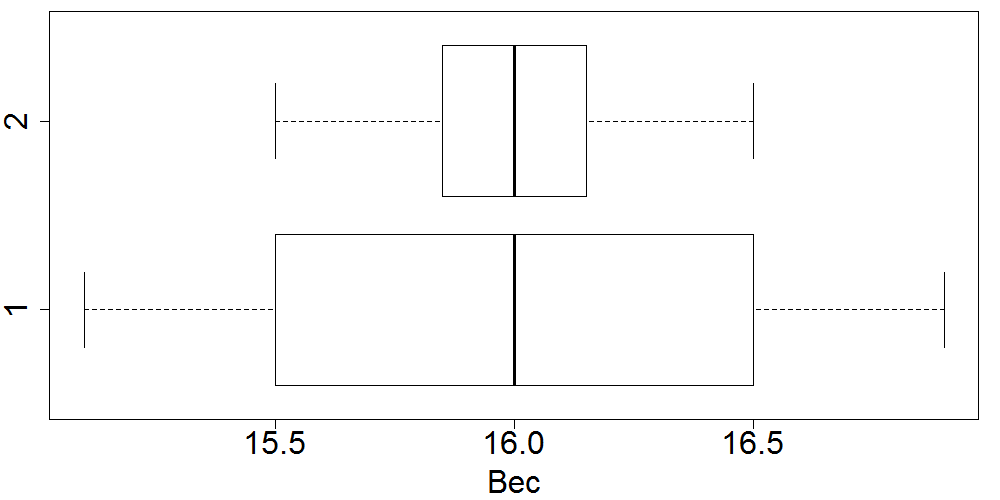
\includegraphics[width=0.4\textwidth]{ingots.png}
    \end{figure} 

    \bigskip

    $H_0\colon$ дисперсия веса слитков не отличается для двух поставщиков.

    $H_1\colon$ дисперсия веса слитков для двух поставщиков отличается $ \Rightarrow p = 0.014$.
}
\end{frame}

\section{Перестановки}
\begin{frame}{Перестановочные критерии}
%%%%%%%%%%%%%%%%%%%%%%%%%%%%%%%%%%%%%%%%%%%%%%%%%%%%%%%%%%%%%%%%%%%%%%%
% При использовании ранговых критериев выборки превращают в ранги, затем делается какое-то дополни- тельное предположение, и на основании этого предположения получается, что разные конфигурации этих рангов при справедливости нулевои? гипотезы могут реализоваться с равнои? вероятностью. Далее необходимо перебрать все конфигурации, и на каждои? посчитать значение статистики — таким образом оценивается ее нулевое распределение.
% Если в этом алгоритме пропустить первыи? пункт (не превращать наблюдения в ранги), а остальное делать точно так же, то получится алгоритм работы перестановочных критериев.
%%%%%%%%%%%%%%%%%%%%%%%%%%%%%%%%%%%%%%%%%%%%%%%%%%%%%%%%%%%%%%%%%%%%%%%
	Ранговые критерии: 
	\begin{enumerate}
		\item выборки $\Rightarrow$ ранги 
        \bigskip
		\item дополнительное предположение (о равенстве распределений / медиан и пр.)
        \bigskip
		\item перестановки  $\Rightarrow$ нулевое распределение статистики
	\end{enumerate}
	
	\bigskip
	
	\textbf{Что если пропустить пункт 1?}
\end{frame}


\begin{frame}
\only<1>{
 \textbf{Пример} (зеркала в клетках мышей):
 
      $H_0\colon$ в клетке с зеркалом мыши проводят в среднем половину времени.
 
      $H_1\colon$ в клетке с зеркалом мыши проводят в среднем не половину времени.
 
      \bigskip
            
Проинтерпретируем задачу по-другому: 

      $H_0\colon$ \textit{матожидание} времени в клетке с зералом равняется 0.5.
 
      $H_1\colon$ \textit{матожидание} времени в клетке с зералом не равняется 0.5
      
}
\only<2>{
\textbf{Предположение:}\\
время, проведенное мышами в клетке с зеркалом симметрично относительно матожидания.

Тогда при верности $H_0$: $X  - 0.5 $ --- симметрично относительно нуля.

\bigskip

\textbf{Статистика:}\\
$T=\sum\limits_{i=1}^n \left(X_i-0.5\right).$

\bigskip

\textbf{Как получить нулевое распределение:}\\
будем переставлять элементы  смещенной выборки $X  - 0.5 $ относительно нуля.
}
\only<3>{
 \textbf{Пример}:
 
      $H_0\colon$ в клетке с зеркалом мыши проводят в среднем половину времени.
 
      $H_1\colon$ в клетке с зеркалом мыши проводят в среднем не половину времени.
 
      \bigskip
 
     Статистика: $T=\sum\limits_{i=1}^n \left(X_i-0.5\right);\;\; t=-0.3784.$
 
     \bigskip
 
     \begin{center}
         \includegraphics[width=0.4\textwidth]{perm_mouse.eps}
     \end{center}
 
     \bigskip
 
     $p=\frac{\#\left[\left|T\right|\geq\left|t\right|\right]}{2^n} = 0.2292.$    
     
     95\% доверительный интервал для доли времени в клетке с зеркалом (BCa бутстреп)~--- $\left[0.447,  0.511\right]$.  
 }
\end{frame}

\subsection{Одна выборка}
\begin{frame}[label=perm1s]{\hyperlink{classification}{\beamerbutton{(8)}} Одновыборочный перестановочный критерий, гипотеза о~среднем}
%%%%%%%%%%%%%%%%%%%%%%%%%%%%%%%%%%%%%%%%%%%%%%%%%%%%%%%%%%%%%%%%%%%%%%%
% Имеется выборка размера n: и делается предположение, что функция распределения F (x) симметрична относительно математического ожидания. Одновыборочныи? перестановочныи? критерии? проверяет нулевую гипотезу о значении математического ожидания случаи?нои? величины, из которои? взята выборка.
% Если нулевая гипотеза этого критерия справедлива, каждыи? из объектов выборки мог с одинаковои? вероятностью реализоваться слева и справа от математического ожидания. Поэтому нужно перебрать все 2n знаков, которые могут стоять в выражении для статистики перед разностью xi?m0. На основании этого перебора и будет восстановлено нулевое распределение статистики.
%%%%%%%%%%%%%%%%%%%%%%%%%%%%%%%%%%%%%%%%%%%%%%%%%%%%%%%%%%%%%%%%%%%%%%%
	\only<1>{
   \begin{center}
     \begin{tabular}{rl}
         выборка:                        & $X_1^n=\left(X_1,\ldots,X_n\right)$\\
					                     & $F\left(X\right)$ симметрично относительно матожидания\\
         нулевая гипотеза:               & $H_0\colon \mathbb{E}X = m_0$ \\
         альтернатива:                   & $H_1\colon \mathbb{E}X <\neq> m_0$ \\
         статистика:                     & $T\left(X^{n}\right) = \sum\limits_{i=1}^n \left(X_i-m_0\right)$ \\
		 нулевое распределение:          & порождается перебором $2^n$ знаков \\
		                                 & перед слагаемыми $X_i-m_0$\\         
     \end{tabular}
 \end{center}

 \bigskip

 Достигаемый уровень значимости~--- доля перестановок знаков, на которых получилось такое же или ещё более экстремальное значение статистики.
 }
 
 \only<2>{
 \textbf{Пример} (диаметры шайб):
 
	Критерий знаковых рангов: 
	\begin{center}
		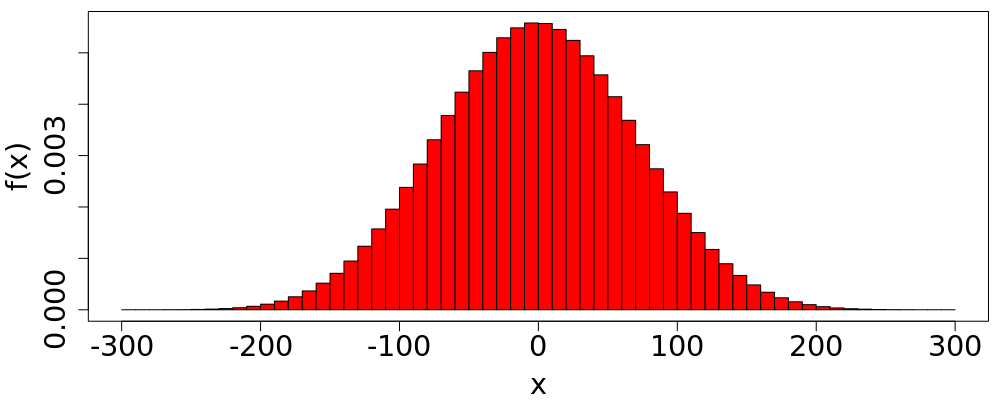
\includegraphics[width=0.35\textwidth]{ranksum24.png}    
	\end{center}	
	\vspace{-10pt}    
	$p=0.0673$
	
	\bigskip
	
	Перестановочный критерий: 
	\begin{center}
		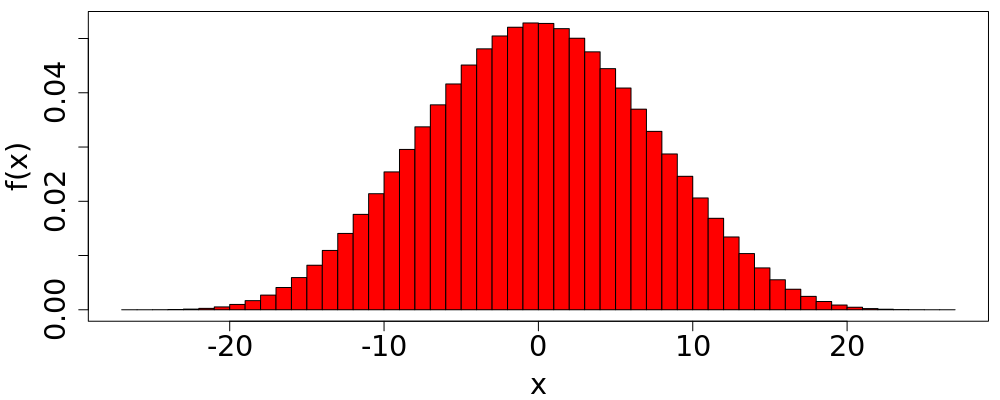
\includegraphics[width=0.35\textwidth]{perm_wash.png}    
	\end{center}	
	\vspace{-10pt}       
	$T=14.6, p=0.1026$
	     
     95\% доверительный интервал для среднего диаметра (BCa бутстреп)~--- $\left[10.11, 11.20\right]$.  
 }
\end{frame}

\subsection{Две выборки}
\begin{frame}[label=perm2ss]{\hyperlink{classification}{\beamerbutton{(9)}} Двухвыборочный перестановочный критерий, гипотеза о средних, связанные выборки}
\only<1>{
   \begin{center}
     \begin{tabular}{rl}
         выборки:                        & $X_1^n=\left(X_{11},\ldots,X_{1n}\right)$\\
		     				             & $X_2^n=\left(X_{21},\ldots,X_{2n}\right)$ \\
								         & выборки связанные\\
								         & распределение попарных разностей симметрично\\
         нулевая гипотеза:               & $H_0\colon \mathbb{E}\left(X_1-X_2\right) = 0$ \\
         альтернатива:                   & $H_1\colon \mathbb{E}\left(X_1-X_2\right) <\neq> 0$ \\
         статистика:                     & $D_i = X_{1i}-X_{2i}$\\
                                         & $T\left(X_1^n, X_2^n\right)  = \sum\limits_{i=1}^n D_i$\\
		 нулевое распределение:          & порождается перебором $2^n$ знаков \\
										 & перед слагаемыми $D_i$\\                                         
     \end{tabular}
 \end{center}
 }
 
 \only<2>{
     \textbf{Пример} (лечение депрессии):
     
	Критерий знаковых рангов: 
	\begin{center}
		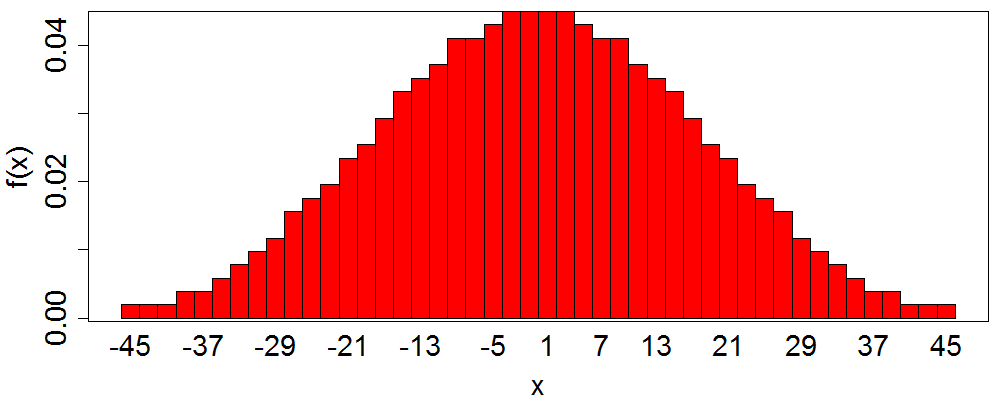
\includegraphics[width=0.35\textwidth]{ranksum9.png}    
	\end{center}	
	\vspace{-10pt}    
	$p = 0.019$
	
	\bigskip
	
	Перестановочный критерий: 
	\begin{center}
		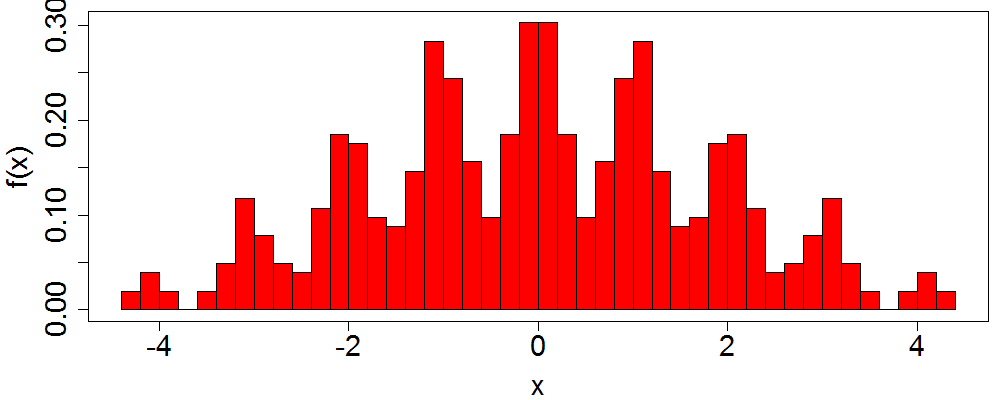
\includegraphics[width=0.35\textwidth]{perm_depr.png}    
	\end{center}	
	\vspace{-10pt}       
	$T= 3.887, p=0.0137$

     95\% доверительный интервал для среднего уменьшения депрессивности (BCa бутстреп)~--- $\left[0.1658, 0.6834\right]$.   
 }
\end{frame}

\begin{frame}[label=perm2sn]{\hyperlink{classification}{\beamerbutton{(10)}} Двухвыборочный перестановочный критерий, гипотеза о средних, независимые выборки}
\only<1>{
%%%%%%%%%%%%%%%%%%%%%%%%%%%%%%%%%%%%%%%%%%%%%%%%%%%%%%%%%%%%%%%%%%%%%%%
% Перестановочныи? критерии? для независимых выборок выглядит абсолютно так же, как критерии? Манна- Уитни за исключением того, что не производятся ранговые преобразования.
%%%%%%%%%%%%%%%%%%%%%%%%%%%%%%%%%%%%%%%%%%%%%%%%%%%%%%%%%%%%%%%%%%%%%%%
\begin{center}
\begin{tabular}{rl}
				выборки:                        & $X_1^{n_1}=\left(X_{11},\ldots,X_{1n_1}\right)$         \\
												& $X_2^{n_2} = \left(X_{21},\ldots,X_{2n_2}\right)$ \\ 
				нулевая гипотеза:               & $H_0\colon F_{X_1}\left(x\right) = F_{X_2}\left(x\right)$ \\
				альтернатива:                   & $H_1\colon F_{X_1}\left(x\right) = F_{X_2}\left(x+\Delta\right), \Delta <\neq> 0$ \\
				статистика:                     & $T\left(X_1^{n_1}, X_2^{n_2}\right) = \frac1{n_1}\sum\limits_{i=1}^{n_1} X_{1i} - \frac1{n_2}\sum\limits_{i=1}^{n_2} X_{2i}$ \\
				нулевое распределение:          & порождается перебором $C_{n_1+n_2}^{n_1}$ \\
												& размещений объединённой выборки\\
			\end{tabular}
 \end{center}
 }
 \only<2>{
     \textbf{Пример} (кофеин и респираторный обмен):
     
	Критерий Манна-Уитни: 
	\begin{center}
		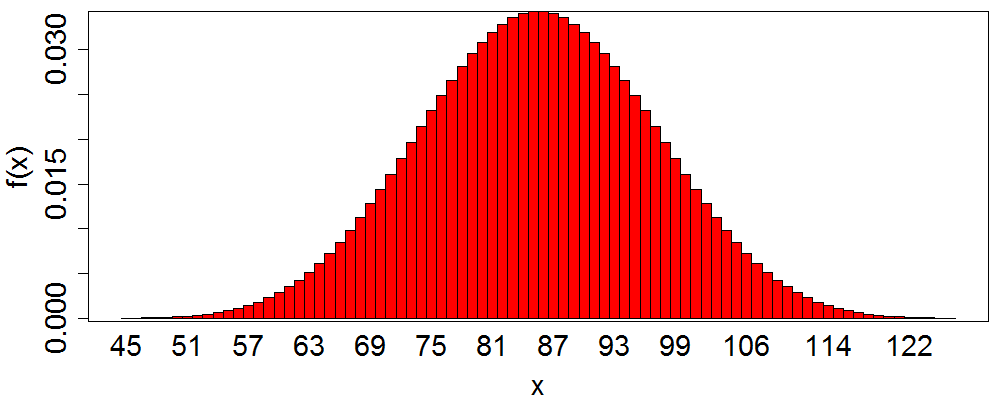
\includegraphics[width=0.35\textwidth]{MU9-9.png}    
	\end{center}	
	\vspace{-10pt}    
	$p=0.0521$
	
	\bigskip
	
	Перестановочный критерий: 
	\begin{center}
		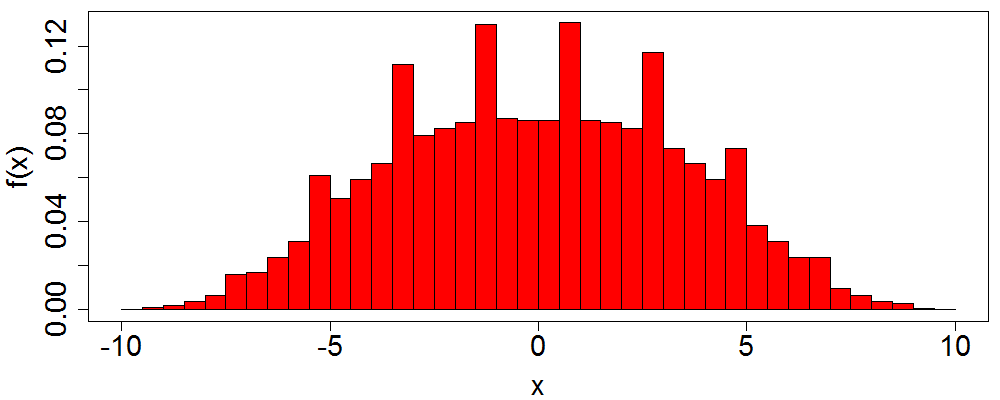
\includegraphics[width=0.35\textwidth]{perm_rer.png}    
	\end{center}	
	\vspace{-10pt}       
	$T= 6.33, p=0.0578$
	 
	 95\% доверительный интервал для разности средних (BCa бутстреп)~--- $\left[1.556, 13.667\right]$.        
 }    
\end{frame}
%%%%%%%%%%%%%%%%%%%%%%%%%%%%%%%%%%%%%%%%%%%%%%%%%%%%%%%%%%%%%%%%%%%%%%%
%Good:  3.7.2.
% Не самый мощный критерий, поскольку (интуитивно) нам пришлось пожертвовать двумя наблюдениями, чтобы перейти к попарными разностям. Аналог этого критерия 
%%%%%%%%%%%%%%%%%%%%%%%%%%%%%%%%%%%%%%%%%%%%%%%%%%%%%%%%%%%%%%%%%%%%%%%
\begin{frame}[label=perm2d] 
\frametitle{\hyperlink{classification}{\beamerbutton{(11)}} Двухвыборочный перестановочный критерий, гипотеза о~дисперсиях, статистика Али}

	\only<1>{
   \begin{center}
     \begin{tabular}{rl}
         выборки:                        & $X_1^{n}=\left(X_{11},\ldots,X_{1n}\right)$\\
                                         & $X_2^{n}=\left(X_{21},\ldots,X_{2n}\right)$ \\
                                         & выборки независимые\\
         нулевая гипотеза:               & $H_0\colon \mathbb{D} X_{1} = \mathbb{D} X_{2}$ \\
         альтернатива:                   & $H_1\colon \mathbb{D} X_{1} <\neq> \mathbb{D} X_{2}$ \\
         статистика:                     &  $\delta\left(D_1^{n-1}\right) = \sum\limits_{i=1}^{n-1} i(n-i)D_{1i},$ \\
					                     & $D_{1i} = X_{1(i+1)} - X_{1(i)}$\\
		нулевое распределение:           & порождается перебором $2^{n-1}$ \\
										 & попарных перестановок $D_{1i}$ и~$D_{2i}$\\					            
     \end{tabular}
 \end{center}
 }
\end{frame}

\begin{frame}{Особенности перестановочных критериев}
%%%%%%%%%%%%%%%%%%%%%%%%%%%%%%%%%%%%%%%%%%%%%%%%%%%%%%%%%%%%%%%%%%%%%%%
% У перестановочных критериев есть некоторые особенности, о которых очень важно помнить.
% Статистику для перестановочных критериев можно выбирать по-разному. В некоторых случаях это приводит к одному и тому же достигаемому уровню значимости, то есть ни на что не влияет. Например, в одновыборочнои? задаче, проверяя гипотезу о равенстве нулю математического ожидания в качестве статистики перестановочного критерия можно использовать как сумму элементов выборки, так и выборочное среднее. Нулевые распределения этих статистик будут отличаться только сдвигом и масштабом, поэтому достигаемыи? уровень значимости, посчитанныи? по ним, будет одним и тем же.
% В других случаях, по-разному выбирая статистику для перестановочного критерия, можно получать разные достигаемые уровни значимости. Например, для статистик ... и ... нулевые распределения отличаются не только сдвигом и масштабом, поэтому достигаемыи? уровень значимости у критериев с этими двумя вариантами статистик тоже будет разныи?. Поэтому при выборе статистики для перестановочного критерия важно думать о том, какие из свои?ств исходнои? случаи?нои? величины для наиболее важны.
% Перестановочные критерии придумал Рональд Фишер еще в начале XX века, однако их начали активно использовать только с появлением и широким распространением компьютеров, потому что для вычисле- ния нулевых распределении? этих критериев используются перестановки. В отличие от ранговых критериев, нормальных аппроксимации? для нулевого распределения в случае больших выборок не существует, поэтому единственныи? способ оценить нулевое распределение статистики — это перебрать много перестановок. По- этому точно посчитать достигаемыи? уровень значимости перестановочного критерия на больших выборках достаточно сложно. Однако его можно посчитать приближе?нно. Для этого нужно взять какое-то случаи?ное подмножество G? множества всех возможных перестановок G. При этом стандартное отклонение достигаемого уровня значимости будет примерно равно   .... На практике, чтобы получить хорошую аппроксимацию достигаемого уровня значимости, достаточно взять несколько тысяч перестановок.
%%%%%%%%%%%%%%%%%%%%%%%%%%%%%%%%%%%%%%%%%%%%%%%%%%%%%%%%%%%%%%%%%%%%%%%
 \begin{itemize}
 \item Статистику критерия можно выбрать разными способами. В~некоторых случаях разные статистики приведут к одному и тому же достигаемому уровню значимости:
 $$X^n, \;\; H_0\colon \mathbb{E}X = 0, \; H_1\colon \mathbb{E}X \neq 0,$$
 $$T_1\left(X^n\right) = \sum\limits_{i=1}^n X_i \;\;\sim \;\; T_2\left(X^n\right) = \bar{X}.$$
 В других случаях достигаемый уровень значимости будет зависеть от выбора статистики:
 $$T_2\left(X^n\right) = \bar{X} \;\; \nsim \;\; T_3\left(X^n\right) = \frac{\bar{X}}{S/\sqrt{n}}.$$
 \item Если множество перестановок $G$ слишком велико, для оценки нулевого распределения $T$ достаточно взять случайное подмножество $G'\in G.$ При этом стандартное отклонение достигаемого уровня значимости будет равно примерно $\sqrt{\frac{p\left(1-p\right)}{\left|G'\right|}}.$
 \end{itemize}
\end{frame}

\subsection{Бутстреп}
\begin{frame}{Перестановки и бутстреп}
%%%%%%%%%%%%%%%%%%%%%%%%%%%%%%%%%%%%%%%%%%%%%%%%%%%%%%%%%%%%%%%%%%%%%%%
% Доверительные интервалы для параметров тесно связаны с проверкои? точечных гипотез об их значениях. Например, z-критерии для средних связаны с нормальными доверительными интервалами, критерии Стьюдента соответствуют доверительным интервалам, построенным с использованием распределения Стьюдента. Для перестановочных критериев ближаи?шим аналогом в мире доверительных интервалов является метод бутстрепа, однако отношения между ними не такие взаимнооднозначные.
% Перестановочные критерии принимают на вход выборку (или выборки), считают на них какую-то статистику. Далее делается дополнительное предположение о распределении, из которого эти выборки взяты. Это пред- положение порождает множество перестановок исходных данных, которые могли реализоваться с одинаковои? вероятностью, если нулевая гипотеза справедлива. На этих перестановках вычисляется значение статистики и таким образом оценивается ее нулевое распределение.
% Бутстреп-методы работают в каком-то смысле похоже. На вход они также принимают выборку или выбор- ки и считают значение статистики, которая оценивает интересующии? параметр. Далее на основании исходных данных генерируется множество бутстреп-псевдовыборок, и на этих псевдовыборках вычисляются значения интересующеи? статистики, то есть оценивается ее распределение.
% Ключевых различии? между этими методами несколько. Во-первых, перестановочныи? критерии? использует дополнительное предположение, которое позволяет породить множество перестановок, которые используются для построения распределения. Во-вторых, перестановки, используемые в перестановочном критерии, — это выборки без возвращения, в то время как бутстреп-методы используют выборки с возвращением (бутстреп- псевдовыборки могут содержать по несколько копии? элементов исходнои? выборки). Кроме того, распреде- ления, которые получаются при использовании этих методов, абсолютно разные, потому что распределение статистики перестановочного критерия — это то распределение, которое статистика будет иметь при спра- ведливости нулевои? гипотезы, в то время как распределение бутстреп-статистики не подразумевает никакои? нулевои? гипотезы.
%%%%%%%%%%%%%%%%%%%%%%%%%%%%%%%%%%%%%%%%%%%%%%%%%%%%%%%%%%%%%%%%%%%%%%%
	Перестановочные критерии:
	\begin{enumerate}
		\item выборки, статистика
		\item дополнительное предположение
		\item перестановки  $\Rightarrow$ нулевое распределение статистики
	\end{enumerate}	
	
	\bigskip	
	
	Бутстреповые доверительные интервалы:
	\begin{enumerate}
		\item выборки, статистика, оценивающая параметр
		\item бутстреп-псевдовыборки  $\Rightarrow$ приближённое распределение статистики
	\end{enumerate}	
\end{frame}

\begin{frame}
%%%%%%%%%%%%%%%%%%%%%%%%%%%%%%%%%%%%%%%%%%%%%%%%%%%%%%%%%%%%%%%%%%%%%%%
% Давайте считать, что мы находимся в реальном мире и доступа к генеральной совокупности у нас нет, а есть только  выборка объёма n. Давайте из этой выборки сделаем много псевдовыборок - выборок с возвращениями - того же самого объёма n. На каждой псевдовыборке посчитаем значение статистики; оказывается, что распределение значений статистики на псевдовыборках часто является хорошей оценкой истинного распределения статистики. Так работает бутстреп (слово означает петлю, которая пришита к заднему краю армейских ботинок, и отсылает нас к выражению "to pull oneself up by one's bootstraps" - что-то вроде Мюнхаузена, вытаскивающего себя из болота за волосы. Действительно, это выглядит как магия.
%%%%%%%%%%%%%%%%%%%%%%%%%%%%%%%%%%%%%%%%%%%%%%%%%%%%%%%%%%%%%%%%%%%%%%%
		\begin{itemize}
			\item бутстреп:
		\end{itemize}	
		\begin{figure}
			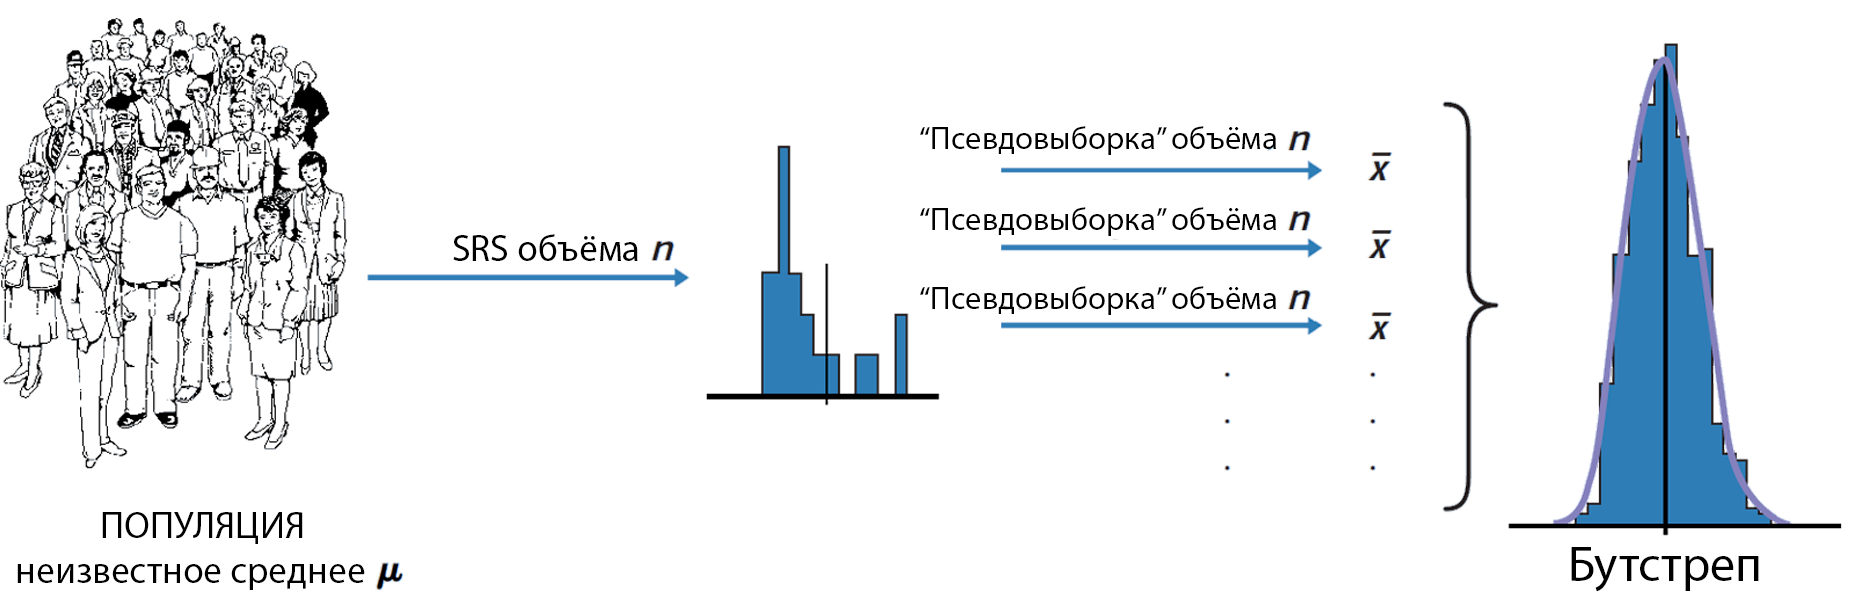
\includegraphics[width=0.8\textwidth]{boot3.png}
		\end{figure}
		Сгенерировать $N$ <<псевдовыборок>> объёма $n$ и оценить выборочное распределение $\hat{\theta}_n$ <<псевдоэмпирическим>>. 
	
\end{frame}
% https://influentialpoints.com/Training/bootstrap_confidence_intervals-principles-properties-assumptions.htm#stud
\begin{frame}
		\begin{itemize}
			
			\item Возьмём выборочные квантили бутстреп-распределения:
			$$\prob\left(\left(F_{\hat{\theta}_n}^{boot}\right)^{-1}\left(\frac{\alpha}{2}\right) \leq \theta \leq \left(F_{\hat{\theta}_n}^{boot}\right)^{-1}\left(1-\frac{\alpha}{2}\right) \right)\approx 1-\alpha.$$	
			Это базовый бутстреп.
			\begin{itemize}
			    \item чем менее симметрично распределение, тем хуже работает метод.
			    \item ошибка аппроксимации обратна корню из мощности выборки ($\prob({\theta}<C_L) = \alpha + \text{Const} \cdot  (n)^{-0.5}.$
			\end{itemize}

\item Посчитаем $S_n^{boot}$~--- выборочное стандартное отклонение $\hat{\theta}_n$ на псевдовыборках; 
			$$\prob \left(\hat{\theta}_n - t_{n-1, 1-\frac{\alpha}{2}} S_n^{boot}  \leq \theta \leq \hat{\theta}_n + t_{n-1, 1-\frac{\alpha}{2}} S_n^{boot}\right)\approx 1-\alpha.$$	
			Это стьюдентизированный бутстреп.
			\begin{itemize}
			    \item имеет меньшую ошибку аппроксимации.
			\end{itemize}
		\end{itemize}
	

\end{frame}

\begin{frame}{BCa}
\small
		\begin{itemize}
			\item Слегка изменим наивный бутстреп:
			$$\prob\left(\left(F_{\hat{\theta}_n}^{boot}\right)^{-1}\left(\alpha_1\right) \leq \theta \leq \left(F_{\hat{\theta}_n}^{boot}\right)^{-1}\left(\alpha_2\right) \right)\approx 1-\alpha,$$	
			
			\vspace{-10pt}
			
			\begin{align*}
			\alpha_1  &= \Phi\left(\hat{z}_0 + \frac{\hat{z}_0 + z_{\frac{\alpha}{2}}}{1 - \hat{a} \left(\hat{z}_0 + z_{\frac{\alpha}{2}}\right)}\right), \\
			\alpha_2  &= \Phi\left(\hat{z}_0 + \frac{\hat{z}_0 + z_{1-\frac{\alpha}{2}}}{1 - \hat{a} \left(\hat{z}_0 + z_{1-\frac{\alpha}{2}} \right)} \right), \\	
			\hat{z}_0 &= \Phi^{-1} \left(\frac1{N} \sum_{i=1}^N \left[ \hat{\theta}_n^{i*} < \hat{\theta}_n\right]\right), \\
			\hat{a}   & \text{ не поместится на этом слайде}.\\
			\end{align*}
			
			\vspace{-5pt}
			
			Это несмещённый ускоренный бутстреп.
		\end{itemize}
	\begin{itemize}
	    \item корректно работает с трансформациями: $C_L(g(\theta)),C_U(g(\theta)) = g(C_L(\theta)), g(C_U(\theta))$.
	    	\begin{itemize}
	    	    \item Как следствие, можно перевести оценку параметра к оценка нормально распределенной случайно величины (Bias correction)
	    	\end{itemize}
	    \item ошибка аппроксимации обратна мощности выборки ($\prob({\theta}<C_L) = \alpha + \text{Const} \cdot (n)^{-1}.$ (Acceleration)
	    
	\end{itemize}
\end{frame}

\begin{frame}{Кофеин и респираторный обмен}
	\only<1>{
%%%%%%%%%%%%%%%%%%%%%%%%%%%%%%%%%%%%%%%%%%%%%%%%%%%%%%%%%%%%%%%%%%%%%%%
% Чтобы лучше это понять, можно вспомнить пример с кофеином и респираторным обменом. В этои? задаче проверялась гипотеза H0 : среднее значение показателя респираторного обмена не отличается в двух группах. Эта нулевая гипотеза проверялась против одностороннеи? альтернативы H1 : под воздеи?ствием кофеина среднее значение показателя респираторного обмена снижается.
% На рисунке 6.16 показано нулевое распределение перестановочного критерия со статистикои? X ?1n ? X ?2n. На рисунке 6.17 — бутстреп-распределение тои? же самои? статистики X ?1n ? X ?2n. Ключевое различие между этими двумя распределениями в том, что они центрированы в разных местах. Перестановочное нулевое рас- пределение центрировано в нуле — значении, соответствующем нулевои? гипотезе. Бутстреп-распределение, в свою очередь, центрировано в выборочном среднем значении? параметра. Параметр в данном случае — это разность средних, то есть центр бутстреп-распределения — это 6.33.
% Для перестановочного критерия доля перестановок, на которых среднее больше либо равно 6.33 (выборочное среднее, которое реализовано в данных) составляет примерно 0.03 (рисунок 6.18). Это и есть достигаемыи? уровень значимости перестановочного критерия, и он точныи?.
% На бутстреп-распределении тои? же самои? статистки доля псевдовыборок, на которых среднее меньше либо равно нулю, составляет 0.011 (рисунок 6.19). Эту величину можно считать приближенным достигаемым уровнем значимости бутстреп-критерия. То есть с помощью доверительных интервалов на основе бутстрепа тоже можно проверять гипотезы, однако нужно это делать немного иначе.
%%%%%%%%%%%%%%%%%%%%%%%%%%%%%%%%%%%%%%%%%%%%%%%%%%%%%%%%%%%%%%%%%%%%%%%
	\begin{figure}
		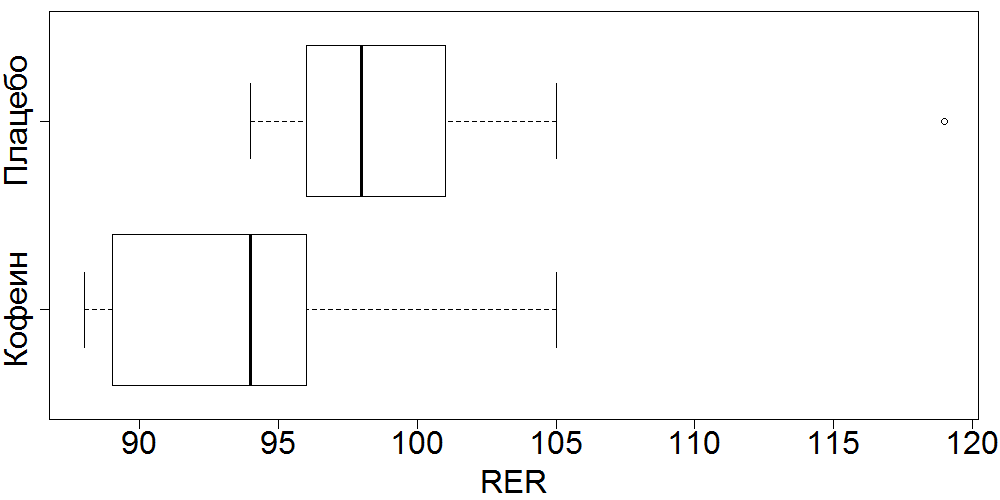
\includegraphics[width=0.5\textwidth]{rer.png}
	\end{figure} 	
	$H_0\colon$ среднее значение показателя респираторного обмена не отличается в~двух группах.
	
	$H_1\colon$ под воздействием кофеина среднее значение показателя респираторного обмена снижается.
	
	$\bar{X}_{1n} - \bar{X}_{2n} = 6.33$
}
\only<2>{
	Нулевое распределение перестановочного критерия со~статистикой $\bar{X}_{1n} - \bar{X}_{2n}$: 
	\begin{center}
		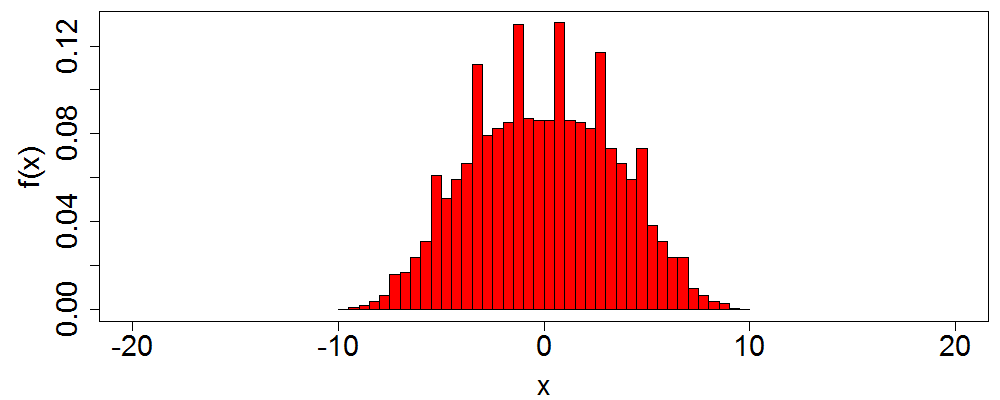
\includegraphics[width=0.5\textwidth]{rer_perm.png}
	\end{center}			
	
	\bigskip
	
	Бутстреп-распределение статистики $\bar{X}_{1n} - \bar{X}_{2n}$:
	\begin{center}
		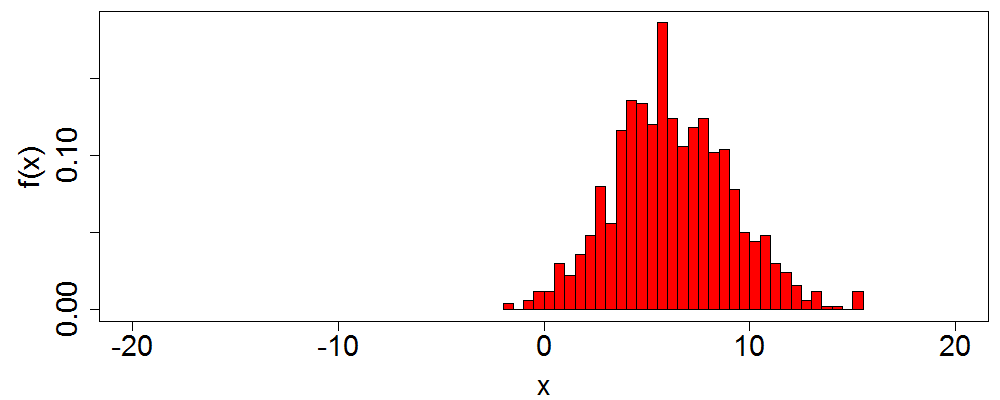
\includegraphics[width=0.5\textwidth]{rer_meanchange_boot.png}    
	\end{center}
}
\only<3>{
	Нулевое распределение перестановочного критерия со~статистикой $\bar{X}_{1n} - \bar{X}_{2n}$: 
	\begin{center}
		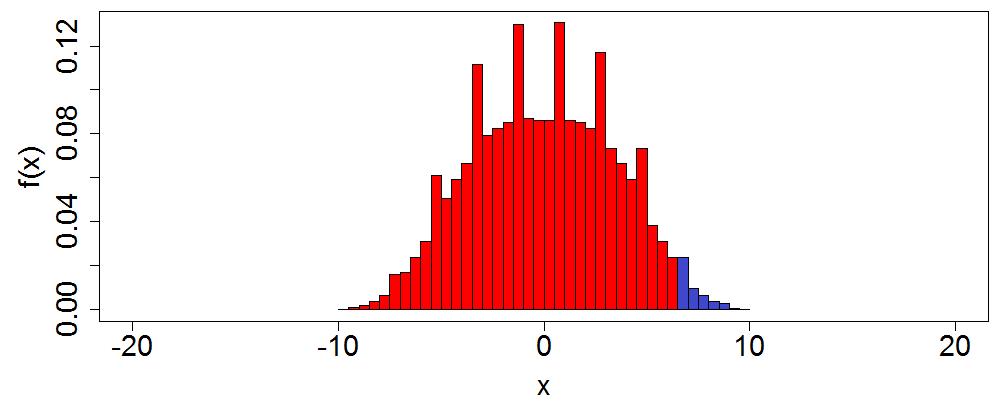
\includegraphics[width=0.8\textwidth]{rer_perm'.png}
	\end{center}		
	
	Доля перестановок, на которых среднее больше либо равно $6.33$~--- $0.0289$.
	
	Это точный достигаемый уровень значимости перестановочного критерия.
}
\only<4>{
	Бутстреп-распределение статистики $\bar{X}_{1n} - \bar{X}_{2n}$:
	\begin{center}
		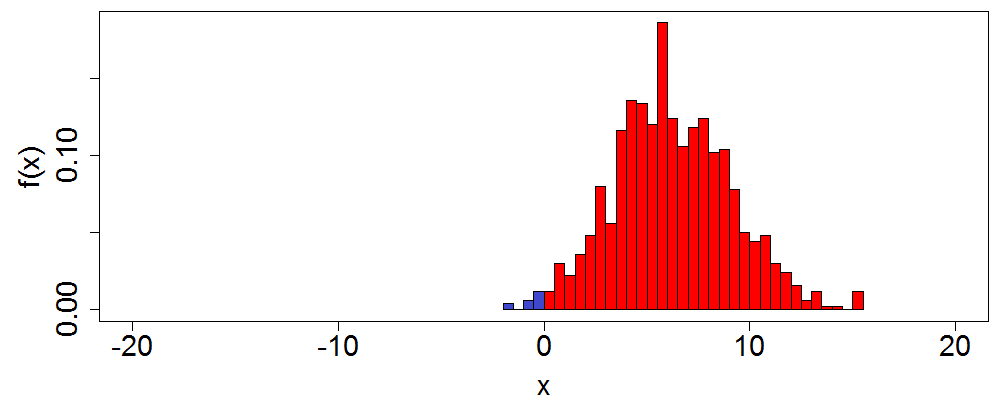
\includegraphics[width=0.8\textwidth]{rer_meanchange_boot'.png}    
	\end{center}		
	
	Доля псевдовыборок, на которых среднее меньше либо равно нулю~--- $0.011$.
	
	Это приближённый достигаемый уровень значимости бутстреп-критерия.	
}
\end{frame}

\begin{frame}{Перестановки vs. бутстреп}	
%%%%%%%%%%%%%%%%%%%%%%%%%%%%%%%%%%%%%%%%%%%%%%%%%%%%%%%%%%%%%%%%%%%%%%%
% Перестановочныи? критерии? с помощью нулевого распределения статистики измеряет расстояние от 0 до D ?n — значения параметра, реализовавшегося в эксперименте. Бутстреп-критерии? измеряет, наоборот, расстояние от D ?n до 0.
% Перестановочныи? критерии? является более точным, потому что в нем перебирается подмножество всех возможных перестановок данных, которые равновероятны при справедливости нулевои? гипотезы. Бутстреп- критерии? в описанном выше виде является только приближенным, поскольку в нем всегда перебирается только конечное подмножество всех возможных бутстреп-псевдовыборок, потому что их заведомо слишком много.
% Самое важное различие между этими двумя критериями заключается в том, что они проверяют разные ги- потезы, поскольку перестановочныи? критерии? использует дополнительные предположения. Перестановочныи? критерии? проверяет гипотезу полного равенства распределении? в двух выборках и проверяется она против альтернативы сдвига (в этом примере одностороннеи?). Предполагается, что никак иначе, кроме как сдвигом, эти распределения отличаться не могут.
% Бутстреп-критерии? проверяет всего лишь гипотезу о равенстве математических ожидании?: Гипотезу равенства он проверяет против одностороннеи? альтернативы точно так же, как и перестановочныи? критерии?. Однако эта гипотеза заведомо более общая: не используется предположение равенстве функции? распределения в двух выборках.
% Проверка гипотез с помощью бутстрепа — это достаточно сложная задача. Показанныи? небольшои? двухвыборочныи? пример позволяет понять плюсы и минусы бутстрепа и перестановочных критериев.
% Бутстреп тоже позволяет проверять гипотезы, приче?м гораздо более широкого класса. Поскольку этот метод не использует дополнительных предположении?, можно проверять только интересующии? параметр (в примере это была разность математических ожидании?). Кроме того, с помощью бутстрепа можно проверять и другие краи?не экзотические гипотезы, которые никакими другими методами проверить нельзя. Например, гипотеза о том, что распределение имеет ровно две моды.
% Если предположения, лежащие в основе перестановочного критерия, выполняются, то перестановочныи? критерии?, во-первых, точнее, поскольку его достигаемыи? уровень значимости точныи?, во-вторых, всегда мощнее, чем аналогичныи? критерии? бутстрепа. Но бутстреп при этом гораздо более гибок, потому что его можно использовать в ситуациях, когда не выполняются предположения, использующиеся в перестановочном критерии.
%%%%%%%%%%%%%%%%%%%%%%%%%%%%%%%%%%%%%%%%%%%%%%%%%%%%%%%%%%%%%%%%%%%%%%%
    \centering
    \begin{tabular}{|c|c|}
    \hline
    \bf Перестановочный критерий & \bf Бутстреп-критерий\\
    \hline
    Центр в нуле & Центр в точечной оценке \\ \hline
    Точный & Приближенный \\ \hline
    $H_0\colon F_{X_1}(x) = F_{X_2}(x)$ & $H_0\colon \mathbb{E}X_1 = \mathbb{E}X_2$ \\ 
    $H_1\colon F_{X_1}(x) = F_{X_2}(x+\Delta), \Delta>0$ & $H_1\colon \mathbb{E}X_1 > \mathbb{E}X_2$\\\hline
    \end{tabular}
	
\end{frame}



\section{Распределения}

\begin{frame}{Различия между моментами высокого порядка}
 \begin{center}
     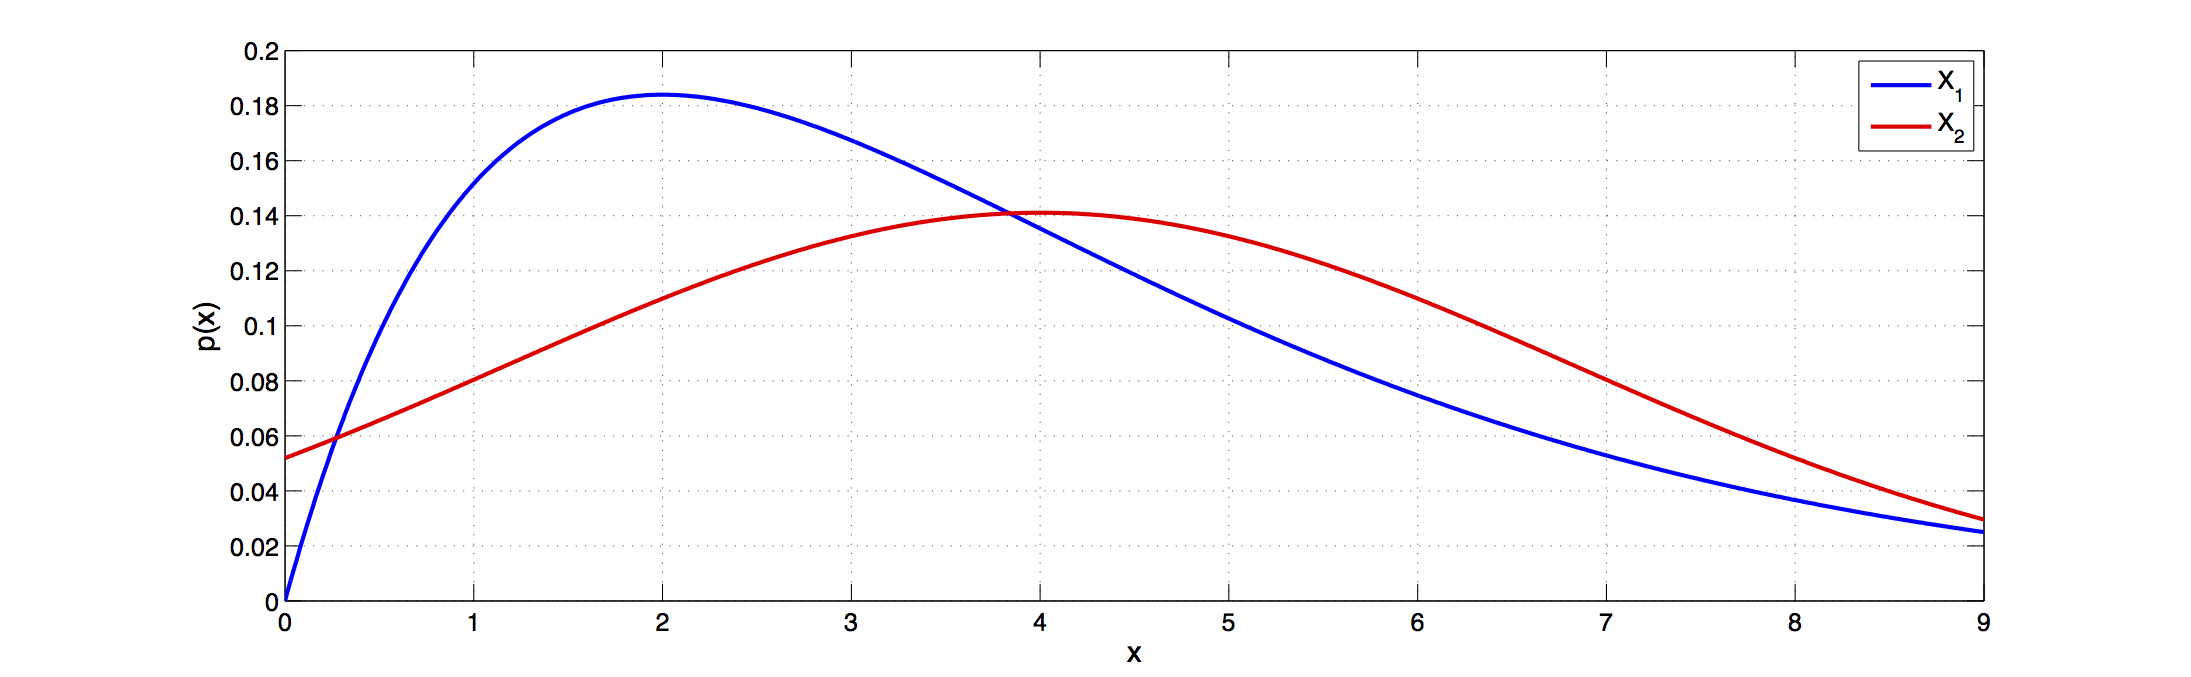
\includegraphics[width=0.8\textwidth,trim=30mm 0mm 30mm 5mm,clip]{distrdiff_example.png}
 \end{center}

 $X_1\sim \chi^2_4, \;\; X_2\sim N\left(4,\sqrt{8}\right);$

 $\mathbb{E}X_1=\mathbb{E}X_2, \;\; \mathbb{D}X_1 = \mathbb{D}X_2.$
\end{frame}

\subsection{Критерии согласия}
%%%%%%%%%%%%%%%%%%%%%%%%%%%%%%%%%%%%%%%%%%%%%%%%%%%%%%%%%%%%%%%%%%%%%%%
% первые два момента распределения - это еще не все распределение. 
% Поэтому при проверке равенства распределений нужно пользоваться другими методами
% Kolmogorov-Smirnov has more power against deviations in the middle, with Cramer-von Mises in between the two (KS and Andersen-Darling) but somewhat more akin to the Kolmogorov-Smirnov in that respect (compared with Anderson-Darling which is missing on the slide)
% Тяжелые хвосты - используетйе АД https://www.researchgate.net/publication/267205556_Power_Comparisons_of_Shapiro-Wilk_Kolmogorov-Smirnov_Lilliefors_and_Anderson-Darling_Tests
%%%%%%%%%%%%%%%%%%%%%%%%%%%%%%%%%%%%%%%%%%%%%%%%%%%%%%%%%%%%%%%%%%%%%%%
\begin{frame}{Двухвыборочные критерии согласия}
   \begin{center}	
     \begin{tabular}{rl}
         выборки:                        & $X_1^{n_1}=\left(X_{11},\ldots,X_{1n_1}\right)$ \\
                                         & $X_2^{n_2}=\left(X_{21},\ldots,X_{2n_2}\right)$ \\
                                         & выборки независимые \\
         нулевая гипотеза:               & $H_0\colon F_{X_1} \left(x\right) = F_{X_2} \left(x\right)$ \\
         альтернатива:                   & $H_1\colon H_0$ неверна \bigskip \\
         \multicolumn{2}{l}{\textbf{Критерий Смирнова}}\\
         статистика:                        & $D\left(X_1^{n_1}, X_2^{n_2}\right) = \sup\limits_{-\infty<x<\infty} \left|F_{n_1X_1} \left(x\right) - F_{n_2 X_2} \left(x\right)\right|$  \bigskip \\
         \multicolumn{2}{l}{\textbf{Критерий Андерсона} (модификация критерия Смирнова-Крамера-}\\
         \multicolumn{2}{l}{фон Мизеса)}\\
         статистика:                        & $T\left(X_1^{n_1}, X_2^{n_2}\right) = \frac1{n_1n_2\left(n_1+n_2\right)} \Biggl( n_1\sum\limits_{i=1}^{n_1} \left(\rank\left(X_{1i}\right) - i\right)^2 + $\\
                                            & \;\;\; $ + n_2 \sum\limits_{j=1}^{n_1} \left(\rank\left(X_{2j}\right) - j\right)^2 \Biggr) - \frac{4n_1n_2-1}{6\left(n_1+n_2\right)}$
     \end{tabular}
 \end{center}

 \bigskip

 Статистики имеют табличные распределения при $H_0$.
\end{frame}

%\subsection{Анализ выживаемости}


\section{}
\begin{frame}{Литература}
 \only<1>{
 \begin{itemize}
 \item критерии знаков (sign tests)~--- Kanji, №№ 45, 46;
 \item критерии знаковых рангов (signed-rank tests)~--- Kanji, №№ 47, 48;
 \item критерий Манна-Уитни-Уилкоксона (Mann-Whitney-Wilcoxon test)~--- Kanji, № 52;
 \item перестановочные критерии (permutation tests)~--- Good, 3.2.1, 3.6.4, 3.7.2 (с ошибкой, исправлено в Ramsey);
 \item двухвыборочные критерии согласия (two-sample goodness-of-fit tests)~--- Кобзарь, 3.1.2.8.
 \end{itemize}

 \bigskip

 {\small
 Кобзарь А.И. \textit{Прикладная математическая статистика}, 2006.
		
	\vspace{5pt}   

	Bonnini S., Corain L., Marozzi M., Salmaso S. \textit{Nonparametric Hypothesis Testing - Rank and Permutation Methods with Applications in R}, 2014.
	
    \vspace{5pt}   

	Shekin D. \textit{Handbook of Parametric and Nonparametric Statistical Procedures}, 2007.
		
    \vspace{5pt}   

    Efron B., Tibshirani R. \textit{An Introduction to the Bootstrap}, 1993.
	\vspace{5pt}
		
	Dinse G.E. (1982). \textit{Nonparametric estimation for partially-complete time and	type of failure data}. Biometrics, 38, 417–431.
		
	\vspace{5pt}

	Good P. \textit{Permutation, Parametric and Bootstrap Tests of Hypotheses: A Practical Guide to Resampling Methods for Testing Hypotheses}, 2005.
 }
	}
	\only<2>{\small    
 Hollander M., Wolfe D.A. \textit{Nonparametric statistical methods}, 1973.	
		
		\vspace{5pt}		    
	
	Kanji G.K. \textit{100 statistical tests}, 2006.
		
		\vspace{5pt}
		    	
	Laureysens I., Blust R., De Temmerman L., Lemmens C., Ceulemans R. (2004). \textit{Clonal variation in heavy metal accumulation and biomass production in a poplar coppice culture. I. Seasonal variation in leaf, wood and bark concentrations.} Environmental Pollution, 131, 485-494.	
		
		\vspace{5pt}
		    	
	Ramsey P.H., Ramsey P.P. (2008). \textit{Brief investigation of tests of variability in the two-sample case}. Journal of Statistical Computation and Simulation, 78(12), 1125--1131.	
		
		\vspace{5pt}
		    	
	Shervin C.M. (2004) \textit{Mirrors as potential environmental enrichment for individually housed laboratory mice}. Applied Animal Behaviour Science, 87(1-2), 95--103.
	}
\end{frame}

\end{document}
